
%Inicio del Preámbulo: Modifícalo bajo tu propio riesgo! Usa los paquetes que requieras para 
%implementar funcionalidades dentro del documento. Se comenta solo lo esencial, puedes buscar los
%paquetes y documentarte de su funcionalidad y puedes eliminarlos también si así lo deseas. 

\documentclass[letterpaper,12pt]{article} %Modifica el tipo de documento y el tamaño de la letra.
\usepackage[utf8]{inputenc} %Formato UTF-8 para caracteres especiales.
\usepackage[shortlabels]{enumitem}
\usepackage[spanish,mexico]{babel} 
\usepackage{amsmath,amssymb,amsfonts,latexsym,cancel}
\usepackage{hyperref}
\usepackage{wrapfig}
\usepackage[rflt]{floatflt}
\usepackage[pdftex]{graphicx}
\usepackage{fancyhdr} %Paquete para el header y el formato de la portada. No sugiero borrarlo!
\usepackage{float}
\usepackage{longtable,multirow,booktabs}
\usepackage{cite}
\usepackage{wrapfig}
\usepackage[square,numbers]{natbib}
\usepackage{multicol}
\usepackage{caption}
\usepackage[]{sidecap}
\usepackage{adjustbox}
\usepackage{parskip}
\usepackage{enumitem}
\usepackage{tikz}
\usepackage{lipsum}
\usepackage[]{xcolor}



%Fin de Préambulo


%Inicio formato de Página. Puedes establecer medidas de la página y modificar el header.

\textheight = 21cm %Medidas de la  página
\textwidth = 18cm  %Medidas de la página
\topmargin = -2cm  %Medidas de la página    
\oddsidemargin = -0.8cm %Medidas de la página
\pagestyle{fancy} %Diseño de la página


\fancyhf{}
\lhead{Facultad de Ingeniería}%%LeftHead
\chead{
\includegraphics[height=1cm]{figures/ORT.png}}%%CenterHead
%\lfoot{USM}
\rhead{Sistemas multiagente}%%RightHead

\setlength{\columnsep}{4mm}%Comandos para el formato de la página.
%\setlength{\parindent}{4em}%Sangría al comenzar un nuevo párrafo.
\setlength{\parindent}{0.5in}
%\setlength{\parindent}{4em}%Sangría al comenzar un nuevo párrafo.
\setlength{\parskip}{1em}%Distancia entre párrafos.
\renewcommand{\baselinestretch}{1.5}% Espacio entre línea y línea o interlineado.
\setlength{\headheight}{33pt}
\fancyfoot[CE,CO]{\\\thepage} %Logo de LaTeX y pie de página.

%Fin formato de Página

%Aquí inicia el documento. Date como magnate
\begin{document}

    %LaTeX te hace el índice automáticamente conforme añades secciones en tu documento.
    \thispagestyle{empty}


\begin{figure}[ht]
    \centering
    
\includegraphics[width=4cm]{figures/ORT.png}
    \label{escudoFI}
\end{figure}
        
\vspace{0.1cm}
    
\begin{center}

    {\scshape\Large Facultad de Ingeniería\par}
    
     {\LARGE Sistemas multiagente}

    % Restauramos el interlineado:
    \begin{center}
        {\LARGE\bfseries Simultaneous Game.\par}

          {\scshape\Large Fecha de entrega: XX/XX/20XX\par}	

        \vspace{2cm}
        \LARGE	{ \textbf{Profesor:}}\\%% \textbf son negritas
        \large		{Marcos Adrian Begerez Oyhenard}
    
          \vspace{-0.5cm}	
        \large		{Martín Iturbide Noria}
    
          \vspace{2cm}	
    
        \LARGE	{ \textbf{Alumno(s):}}\\%% \textbf son negritas

        \normalsize	 {Natalia Campiglia - 349251}
        
        \vspace{-0.5cm}
        
        \normalsize		{Marcos Mussio - 362839 }
        
        \vspace{-0.5cm}

            
    \end{center}

\end{center}
    \newpage
    \tableofcontents
    \newpage


\section{Introducción}

Los sistemas multiagente (Multi-Agent Systems, MAS) constituyen un área de estudio de la inteligencia artificial enfocada en escenarios donde múltiples agentes autónomos interactúan dentro de un ambiente compartido para alcanzar determinados objetivos. Estos agentes pueden colaborar, competir o mantener objetivos parcialmente alineados, generando dinámicas complejas de coordinación y toma de decisiones. En este contexto, el aprendizaje por refuerzo multiagente (Multi-Agent Reinforcement Learning, MARL) surge como una extensión del aprendizaje por refuerzo tradicional, permitiendo que varios agentes aprendan simultáneamente mediante interacción repetida con el ambiente y entre ellos.

En MARL, cada agente observa el estado del entorno, ejecuta acciones y recibe recompensas que guían el proceso de aprendizaje. Sin embargo, a diferencia del caso single-agent, la presencia de múltiples agentes introduce desafíos adicionales, tales como la no estacionariedad del entorno, la necesidad de coordinación y la existencia de equilibrios estratégicos. Debido a esto, muchos algoritmos de aprendizaje multiagente combinan conceptos provenientes tanto del aprendizaje por refuerzo como de la teoría de juegos.

El objetivo de este trabajo es implementar y analizar distintos algoritmos clásicos de aprendizaje multiagente, evaluando su comportamiento en diversos ambientes competitivos y cooperativos. En particular, se implementaron los siguientes algoritmos:

\begin{itemize}
    \item Fictitious Play (FP)
    \item Regret Matching (RM)
    \item Independent Q-Learning (IQL)
    \item Joint-Action Learning with Agent Modeling (JAL-AM)
\end{itemize}

De acuerdo con la consigna del obligatorio, los algoritmos fueron validados utilizando diferentes ambientes de prueba, incluyendo Matching Pennies, Rock-Paper-Scissors (RPS), Blotto y Foraging. Asimismo, se realizaron múltiples experimentos enfrentando distintos agentes entre sí, por ejemplo FP vs FP, FP vs RM e IQL vs IQL, con el objetivo de analizar propiedades como convergencia, estabilidad, capacidad de coordinación y adaptación estratégica.

Los ambientes seleccionados permiten estudiar diferentes tipos de interacción multiagente. Juegos como Matching Pennies y Rock-Paper-Scissors representan escenarios competitivos de suma cero donde el equilibrio de Nash juega un rol central, mientras que ambientes como Foraging permiten analizar problemas de cooperación y coordinación entre múltiples agentes.

El informe se encuentra organizado de la siguiente manera. En primer lugar, se presenta el marco teórico necesario sobre sistemas multiagente, aprendizaje por refuerzo y teoría de juegos. Luego, se describen los algoritmos implementados y los ambientes utilizados. Posteriormente, se detallan los aspectos de implementación y el diseño experimental empleado para evaluar los algoritmos. Finalmente, se presentan y analizan los resultados obtenidos, discutiendo las fortalezas y limitaciones observadas en cada enfoque.

\section{Marco Teórico}

\subsection{Aprendizaje por Refuerzo Multiagente}

El aprendizaje por refuerzo multiagente (Multi-Agent Reinforcement Learning, MARL) estudia escenarios donde múltiples agentes aprenden simultáneamente mediante interacción con un ambiente compartido. Cada agente observa el estado del entorno, ejecuta acciones y recibe recompensas que guían su aprendizaje.

A diferencia del aprendizaje por refuerzo tradicional, en MARL el entorno se vuelve no estacionario, ya que las políticas de los demás agentes cambian durante el entrenamiento.

\subsection{Juegos Simultáneos}

En este trabajo se consideran principalmente juegos simultáneos, donde todos los agentes seleccionan sus acciones al mismo tiempo.

Un juego puede representarse mediante:

\[
G = (I, A, R)
\]

\begin{itemize}
    \item $I$ es el conjunto de jugadores.
    \item $A$ representa las acciones disponibles.
    \item $R$ representa las recompensas asociadas a las acciones conjuntas.
\end{itemize}

\subsubsection{Equilibrio de Nash}

Un equilibrio de Nash corresponde a una estrategia conjunta donde ningún jugador puede mejorar su recompensa modificando unilateralmente su estrategia.

\[
\forall i \in I : \pi_i^* \in BR_i(\pi_{-i}^*)
\]

En juegos como Matching Pennies y Rock-Paper-Scissors, el equilibrio se encuentra en estrategias mixtas.

\subsection{Fictitious Play}

Fictitious Play (FP) es un algoritmo donde cada agente estima las estrategias de los demás jugadores a partir de las acciones observadas previamente y responde utilizando una mejor respuesta.

\subsection{Regret Matching}

Regret Matching (RM) es un algoritmo basado en el concepto de arrepentimiento (regret). Las probabilidades de seleccionar acciones aumentan para aquellas acciones que hubieran generado mejores recompensas en iteraciones anteriores.

\subsection{Independent Q-Learning}

Independent Q-Learning (IQL) aplica Q-Learning de manera independiente para cada agente.

La actualización de la función Q se realiza mediante:

\[
Q(s,a) \leftarrow Q(s,a) +
\alpha
\left[
r + \gamma \max_{a'} Q(s',a') - Q(s,a)
\right]
\]

\subsection{Joint-Action Learning with Agent Modeling}

Joint-Action Learning with Agent Modeling (JAL-AM) extiende Q-Learning incorporando modelos sobre las acciones de los demás agentes, aprendiendo valores asociados a acciones conjuntas.

\[
Q(s,a_i,a_{-i})
\]

\section{Ambientes}

Con el objetivo de evaluar el comportamiento de los algoritmos implementados, se realizaron experimentos sobre distintos ambientes competitivos y cooperativos. Cada ambiente presenta características diferentes, permitiendo analizar propiedades como convergencia, estabilidad, adaptación estratégica y coordinación entre agentes.

\subsection{Matching Pennies}

Matching Pennies es un juego competitivo de suma cero para dos jugadores. Cada jugador debe elegir simultáneamente entre dos acciones: \textit{Heads} o \textit{Tails}.

Si ambos jugadores seleccionan la misma acción, el jugador 1 obtiene una recompensa positiva y el jugador 2 una recompensa negativa. En caso contrario, ocurre lo inverso.

La matriz de pagos utilizada es la siguiente:

\[
\begin{array}{c|cc}
 & H & T \\
\hline
H & (1,-1) & (-1,1) \\
T & (-1,1) & (1,-1)
\end{array}
\]

Este ambiente resulta útil para analizar convergencia hacia estrategias mixtas y equilibrio de Nash.


\subsection{Rock-Paper-Scissors}

Rock-Paper-Scissors (RPS) es un juego simultáneo de suma cero donde cada jugador puede seleccionar una de tres acciones: Rock, Paper o Scissors.

Las reglas son las siguientes:

\begin{itemize}
    \item Rock vence a Scissors.
    \item Scissors vence a Paper.
    \item Paper vence a Rock.
\end{itemize}

La matriz de recompensas utilizada es:

\[
\begin{array}{c|ccc}
 & R & P & S \\
\hline
R & (0,0) & (-1,1) & (1,-1) \\
P & (1,-1) & (0,0) & (-1,1) \\
S & (-1,1) & (1,-1) & (0,0)
\end{array}
\]

El equilibrio de Nash de este juego corresponde a una estrategia mixta uniforme.


\subsection{Blotto}

Blotto es un juego estratégico donde los agentes deben distribuir recursos limitados entre múltiples campos de batalla. Cada campo es ganado por el jugador que asigna mayor cantidad de recursos.

El objetivo consiste en maximizar la cantidad de campos ganados o la recompensa total obtenida.

Este ambiente introduce un espacio de acciones más complejo que Matching Pennies y RPS, permitiendo analizar la capacidad de exploración y adaptación estratégica de los algoritmos.


\subsection{Foraging}

Foraging es un ambiente multiagente secuencial en el que varios agentes se desplazan dentro de una grilla para recolectar comida. En cada paso, los agentes observan el estado del entorno, eligen una acción de movimiento o la acción \texttt{LOAD}, y reciben recompensa cuando el recurso es recolectado. A diferencia de juegos matriciales como Matching Pennies o RPS, aquí las decisiones no dependen solamente de una acción simultánea aislada, sino también de la posición de los agentes, la ubicación de la comida y la historia del episodio.

El ambiente permite estudiar coordinación, competencia por recursos escasos y cooperación. En las configuraciones no cooperativas, puede ocurrir que un agente llegue antes a la comida y concentre una mayor parte de la recompensa. En las configuraciones cooperativas, en cambio, los agentes deben coordinar sus posiciones y acciones para recolectar el recurso, por lo que el desempeño individual depende más fuertemente del comportamiento conjunto.

\begin{table}[H]
    \centering
    \begin{adjustbox}{max width=\textwidth}
    \begin{tabular}{lllll}
        \toprule
        Configuración & Mapa & Agentes & Comida & Característica principal \\
        \midrule
        \texttt{Foraging-5x5-2p-1f-v3} & $5 \times 5$ & 2 & 1 & Escenario pequeño, exploración simple. \\
        \texttt{Foraging-8x8-2p-1f-v3} & $8 \times 8$ & 2 & 1 & Mayor espacio de estados y trayectorias más largas. \\
        \texttt{Foraging-8x8-3p-1f-v3} & $8 \times 8$ & 3 & 1 & Más agentes compiten o se coordinan alrededor del mismo recurso. \\
        \texttt{Foraging-8x8-3p-1f-coop-v3} & $8 \times 8$ & 3 & 1 & Modo cooperativo, requiere coordinación para recolectar. \\
        \bottomrule
    \end{tabular}
    \end{adjustbox}
    \caption{Configuraciones evaluadas del ambiente Foraging.}
\end{table}

La evaluación de Foraging se basa principalmente en métricas de desempeño: recompensa promedio por episodio, tasa de éxito, cantidad promedio de pasos hasta recolectar la comida y distribución de recompensas entre agentes.

Además, como es un juego multiagente, también interesa analizar la estabilidad de las políticas aprendidas en relación con el equilibrio de Nash. En este caso no hay un equilibrio simple y conocido como en RPS, porque el juego tiene estados y se desarrolla a lo largo de varios pasos. Por eso, se evalúa de forma empírica si los agentes logran coordinarse y si alguno podría mejorar claramente cambiando su política mientras los demás mantienen la suya.


\subsection{Cournot}

Cournot es un juego económico simultáneo donde dos o más empresas compiten eligiendo la cantidad de producto que desean producir. Todas las empresas toman su decisión al mismo tiempo y, una vez definidas las cantidades, el precio de mercado se determina en función de la producción total.

En general, si la producción total aumenta, el precio de mercado disminuye. Por lo tanto, cada agente debe decidir cuánto producir considerando tanto su propio beneficio como el impacto de las decisiones de los demás agentes.

Este ambiente permite analizar comportamientos estratégicos en juegos de competencia económica, donde los agentes buscan maximizar su ganancia individual.

\subsection{Chicken}

El juego de \textit{Chicken} es un juego clásico de conflicto donde dos agentes tienen incentivos a ser agresivos, pero si ambos son agresivos al mismo tiempo, el resultado es muy malo para los dos.

La idea típica es:

\begin{quote}
Dos autos van uno hacia el otro.\\
Cada conductor puede mantenerse firme o desviarse.\\
Si uno se desvía y el otro no, el que no se desvía ``gana''.\\
Si ambos se desvían, nadie gana del todo, pero evitan el choque.\\
Si ninguno se desvía, chocan, que es el peor resultado para ambos.
\end{quote}

\subsection{Battle of sexes}
Es un juego en donde los jugadores deben elegir entre ir al \textbf{Cine} o a un \textbf{Partido} de fútbol. Prefieren ir juntos, pero \texttt{agent\_0} prefiere el Cine y \texttt{agent\_1} el Partido.

\textbf{A diferencia de Matching Pennies y Blotto, este juego NO es de suma cero}: ambos jugadores pueden obtener utilidad positiva simultáneamente.

Matrices de utilidades $(u_0, u_1)$, donde las filas corresponden a \texttt{agent\_0} y las columnas a \texttt{agent\_1}:

\[
\begin{array}{c|cc}
 & \textbf{Cine} & \textbf{Partido} \\
\hline
\textbf{Cine} & (2,1) & (0,0) \\
\textbf{Partido} & (0,0) & (1,2)
\end{array}
\]

\texttt{agent\_0} obtiene más utilidad coordinando en Cine; \texttt{agent\_1}, coincidiendo en Partido. La descoordinación da $0$ a ambos.

\section{Experimentos}


Para evaluar el desempeño de los algoritmos implementados, se realizaron experimentos sobre cada uno de los ambientes descritos anteriormente. En todos los casos se utilizaron 20.000 episodios por experimento y 10 semillas aleatorias distintas, con el objetivo de obtener estimaciones estadísticamente robustas. Los resultados se presentan como el promedio sobre las semillas, acompañado de intervalos de confianza del 95\%.

\subsection{Rock-Paper-Scissors}

Rock-Paper-Scissors (RPS) es un juego de suma cero con dos agentes y tres acciones posibles: Rock (R), Paper (P) y Scissors (S). El único equilibrio de Nash del juego corresponde a la estrategia mixta uniforme $\pi^* = (1/3,\, 1/3,\, 1/3)$ para ambos jugadores.

Para analizar el comportamiento de los algoritmos en este ambiente, se ejecutaron experimentos de \textit{self-play} enfrentando a cada algoritmo consigo mismo, así como experimentos de \textit{cross-play} enfrentando algoritmos distintos entre sí y contra un agente aleatorio (Random).



\subsubsection*{FP vs FP}

\begin{figure}[H]
    \centering
    
\includegraphics[width=\textwidth]{figures/RPS/fp_vs_fp.png}
    \caption{FP vs FP en RPS.}
\end{figure}

\begin{figure}[H]
    \centering
    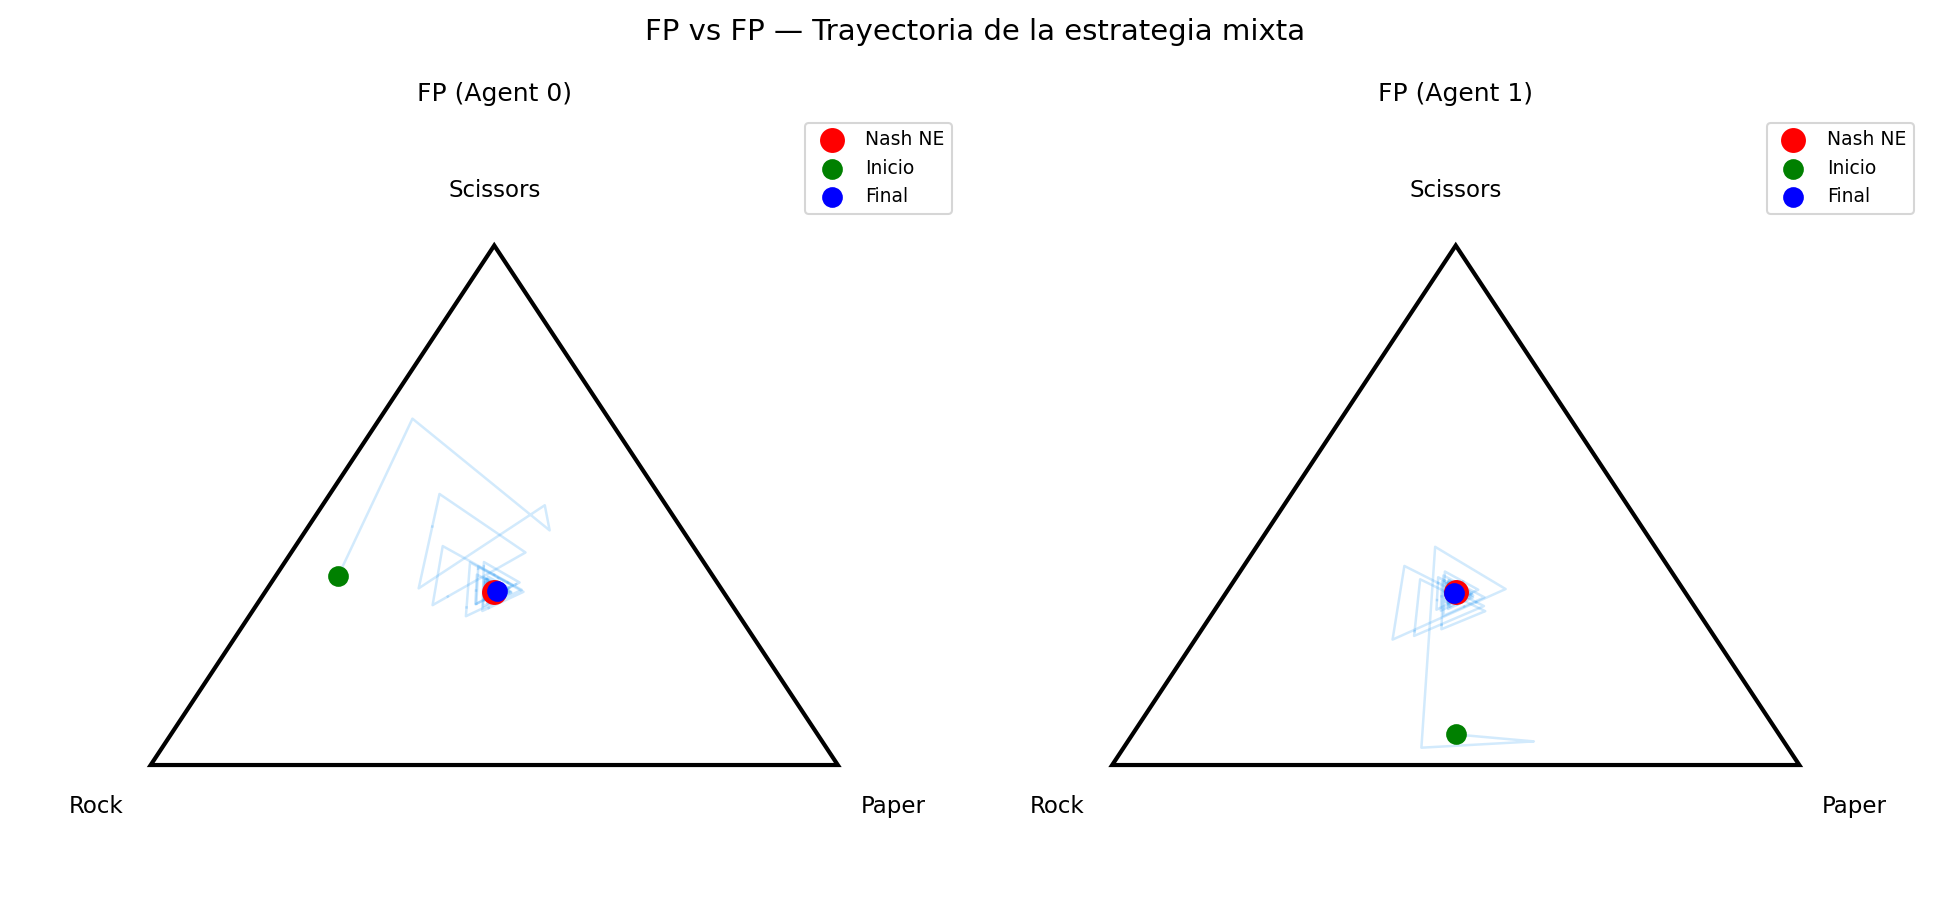
\includegraphics[width=\textwidth]{figures/RPS/simplex_fp_vs_fp.png}
    \caption{Trayectoria de políticas para FP vs FP.}
\end{figure}

En self-play, FP muestra el comportamiento clásico esperado en RPS. Las recompensas oscilan alrededor de cero durante todo el entrenamiento, algo consistente con un juego de suma cero donde ningún agente puede explotar sistemáticamente al otro.

La política instantánea nunca converge completamente, sino que continúa oscilando alrededor del equilibrio de Nash. Sin embargo, la política promedio acumulada sí converge claramente hacia $(1/3,1/3,1/3)$.

Esto también puede observarse en las trayectorias de la política: ambos agentes generan espirales alrededor del centro del triángulo y terminan estabilizándose cerca del equilibrio mixto.

\subsubsection*{RM vs RM}

\begin{figure}[H]
    \centering
    
\includegraphics[width=\textwidth]{figures/RPS/rm_vs_rm.png}
    \caption{RM vs RM en RPS.}
\end{figure}

\begin{figure}[H]
    \centering
    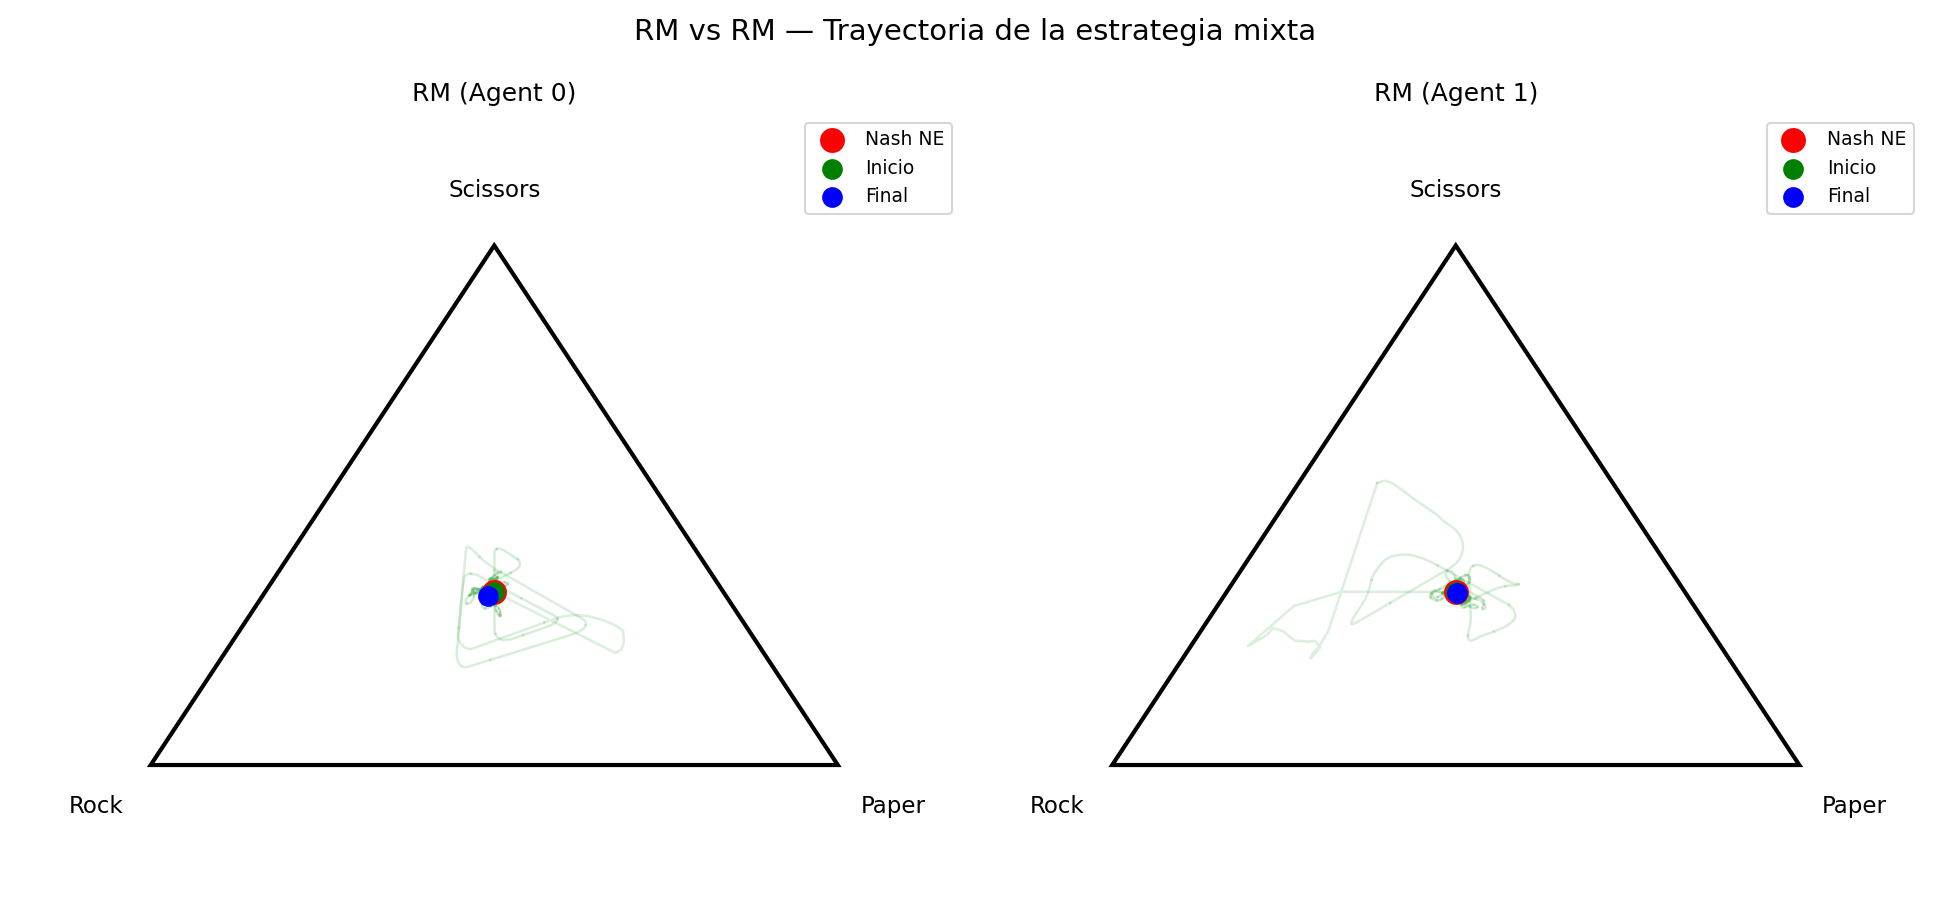
\includegraphics[width=\textwidth]{figures/RPS/simplex_rm_vs_rm.png}
    \caption{Trayectoria de políticas para RM vs RM en el simplex.}
\end{figure}

RM mostró un comportamiento todavía más estable que FP. Las oscilaciones de la política instantánea son menores y la política promedio acumulada converge rápidamente hacia el equilibrio de Nash.

En el trayectoria de la política, se observa que las trayectorias permanecen mucho más concentradas cerca del centro, reflejando la propiedad de no-arrepentimiento del algoritmo.

\subsubsection*{IQL vs IQL}

\begin{figure}[H]
    \centering
    
\includegraphics[width=\textwidth]{figures/RPS/iql_vs_iql.png}
    \caption{IQL vs IQL en RPS.}
\end{figure}

\begin{figure}[H]
    \centering
    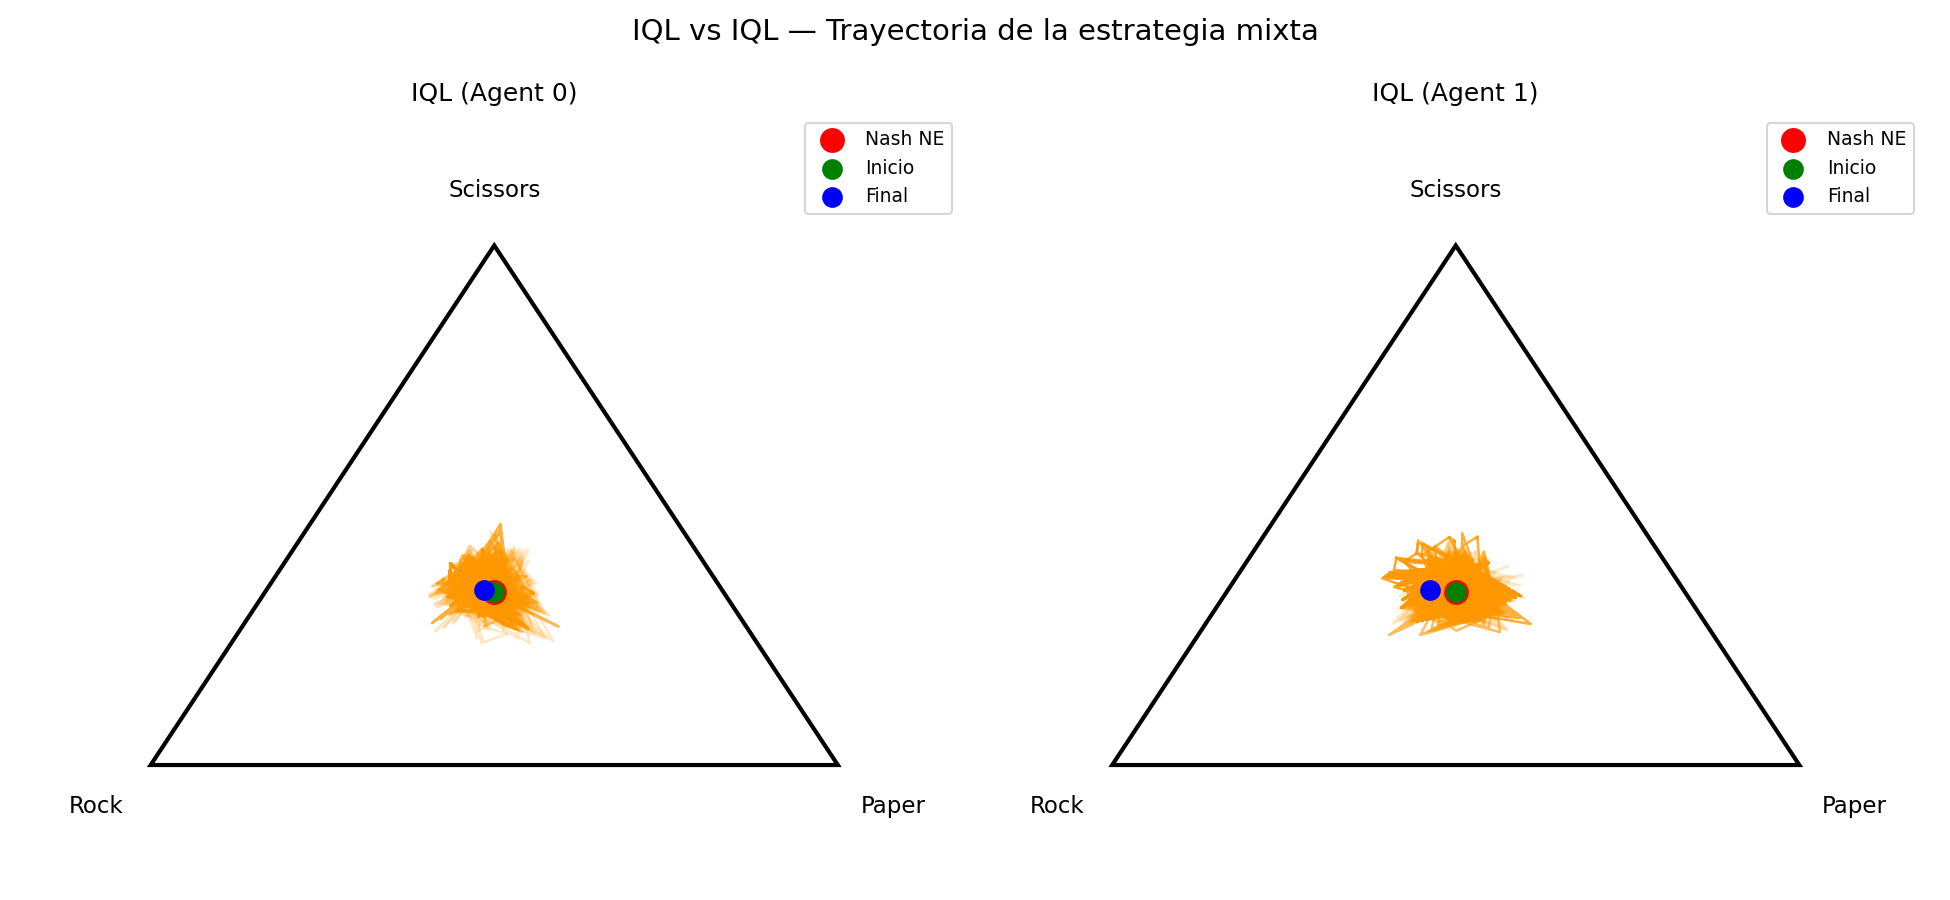
\includegraphics[width=\textwidth]{figures/RPS/simplex_iql_vs_iql.png}
    \caption{Trayectoria de políticas para IQL vs IQL en el simplex.}
\end{figure}

IQL fue el algoritmo más inestable en RPS. Aunque la política promedio acumulada logra acercarse parcialmente al equilibrio de Nash, la política instantánea presenta fluctuaciones importantes durante todo el entrenamiento.

Esto ocurre porque cada agente aprende asumiendo que el entorno es estacionario, cuando en realidad la política del oponente cambia continuamente.

Las trayectorias en el simplex son considerablemente más erráticas que en FP o RM, mostrando movimientos bruscos y una mayor dispersión alrededor del equilibrio.

Aun así, el promedio acumulado termina relativamente cerca de $(1/3,1/3,1/3)$, aunque con bastante más varianza.

\subsubsection*{JAL-AM vs JAL-AM}

\begin{figure}[H]
    \centering
    
\includegraphics[width=\textwidth]{figures/RPS/jalam_vs_jalam.png}
    \caption{JAL-AM vs JAL-AM en RPS.}
\end{figure}

\begin{figure}[H]
    \centering
    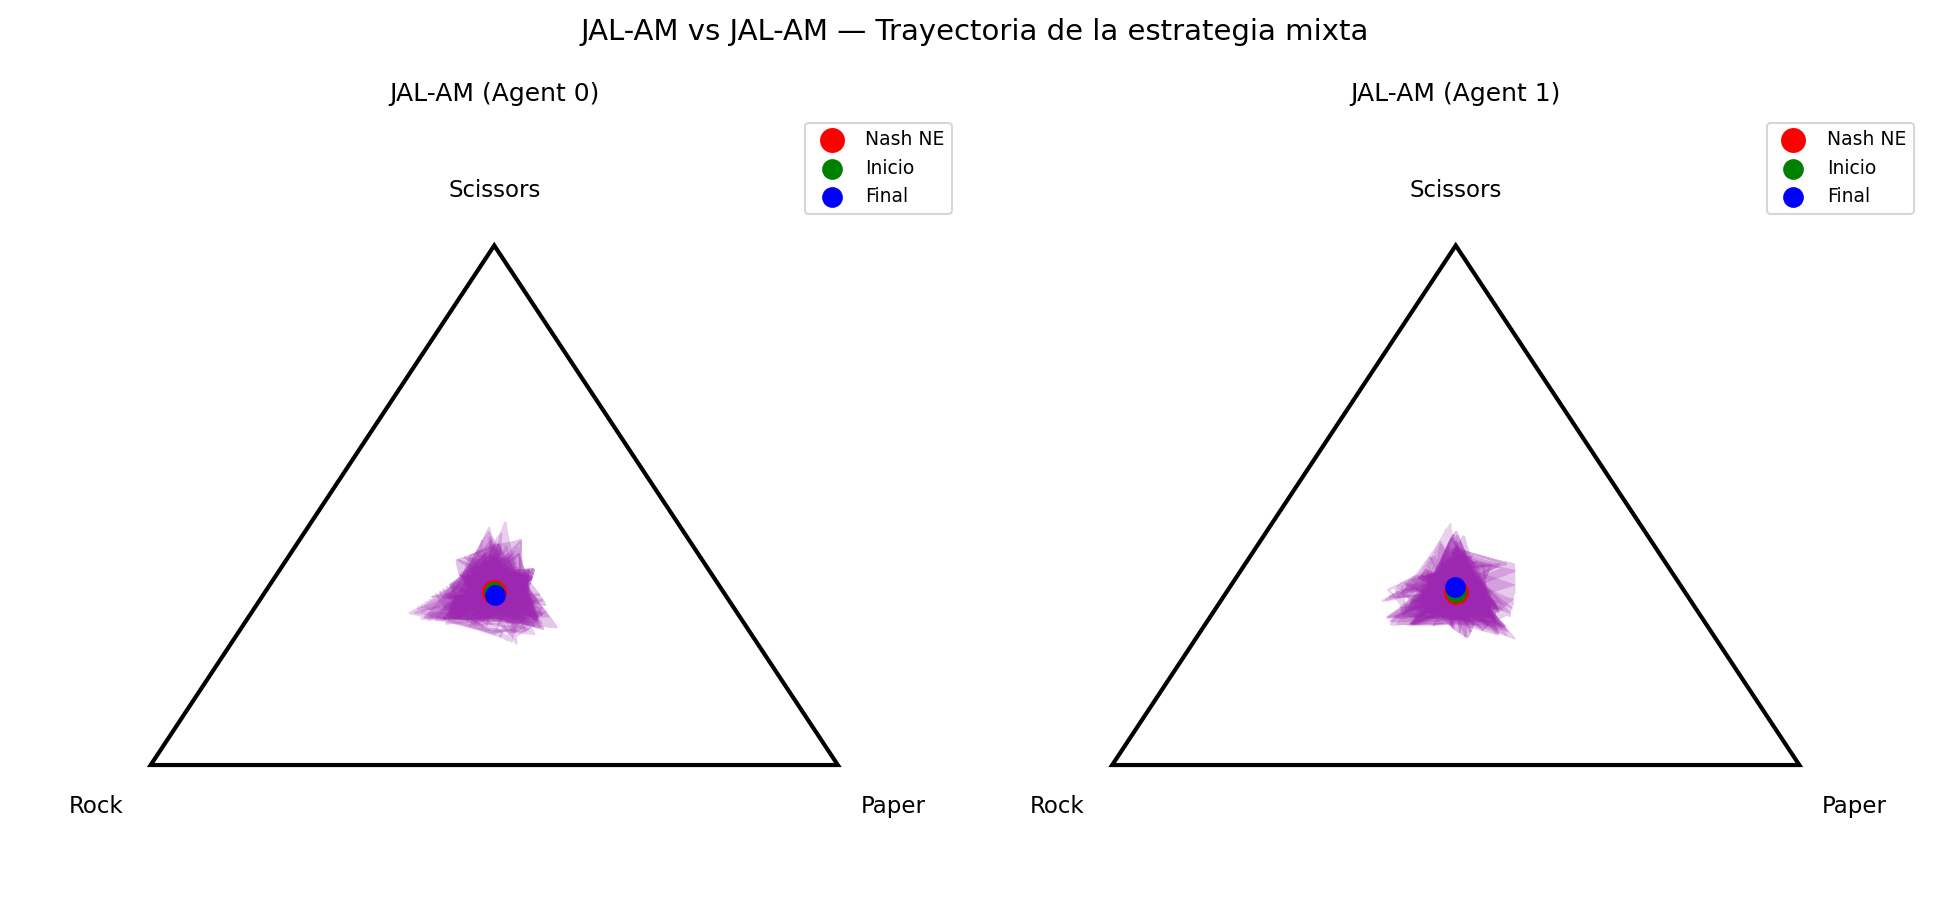
\includegraphics[width=\textwidth]{figures/RPS/simplex_jalam_vs_jalam.png}
    \caption{Trayectoria de políticas para JAL-AM vs JAL-AM en el simplex.}
\end{figure}

JAL-AM obtuvo resultados considerablemente mejores que IQL. Al incorporar modelado explícito de las acciones del oponente, el algoritmo logra reducir parcialmente los efectos de la no estacionariedad.

Las oscilaciones de la política instantánea son menores y la política promedio acumulada converge más rápidamente hacia $(1/3, 1/3, 1/3)$ que en IQL. Además, la trayectoria de la estrategia mixta evidencia una mayor concentración alrededor del equilibrio, aunque todavía con más variabilidad que FP o RM.

De todas formas, no se esperaba que JAL-AM tenga un comportamiento perfectamente estable en RPS, dado que Rock-Paper-Scissors es un juego de suma cero donde la mejor respuesta cambia constantemente dependiendo de la política del oponente. En este tipo de entornos, modelar al oponente no garantiza convergencia estable, ya que ambos agentes continúan adaptándose mutuamente todo el tiempo.

Por lo tanto, el hecho de que JAL-AM siga mostrando oscilaciones y trayectorias que orbitan alrededor del equilibrio, sin converger completamente en política instantánea, era un resultado esperable. Aun así, el algoritmo logra mantenerse más cerca del equilibrio que IQL, dado que JAL-AM intenta estimar qué acciones está realizando el oponente y utiliza esa información para actualizar sus valores de manera más informada. Aunque esto no elimina completamente la no estacionariedad, sí permite reducir parcialmente su impacto. 

En cambio en IQL, cada agente actualiza sus valores Q asumiendo que las probabilidades de transición y recompensa no cambian. Sin embargo, en un entorno multiagente esto no se cumple, ya que el oponente también está aprendiendo y modificando continuamente su política. Esto provoca que los valores Q se vuelvan inestables y que la política oscile constantemente.




\subsubsection*{FP vs RM}

\begin{figure}[H]
    \centering
    
\includegraphics[width=\textwidth]{figures/RPS/fp_vs_rm.png}
    \caption{FP vs RM en RPS.}
\end{figure}

\begin{figure}[H]
    \centering
    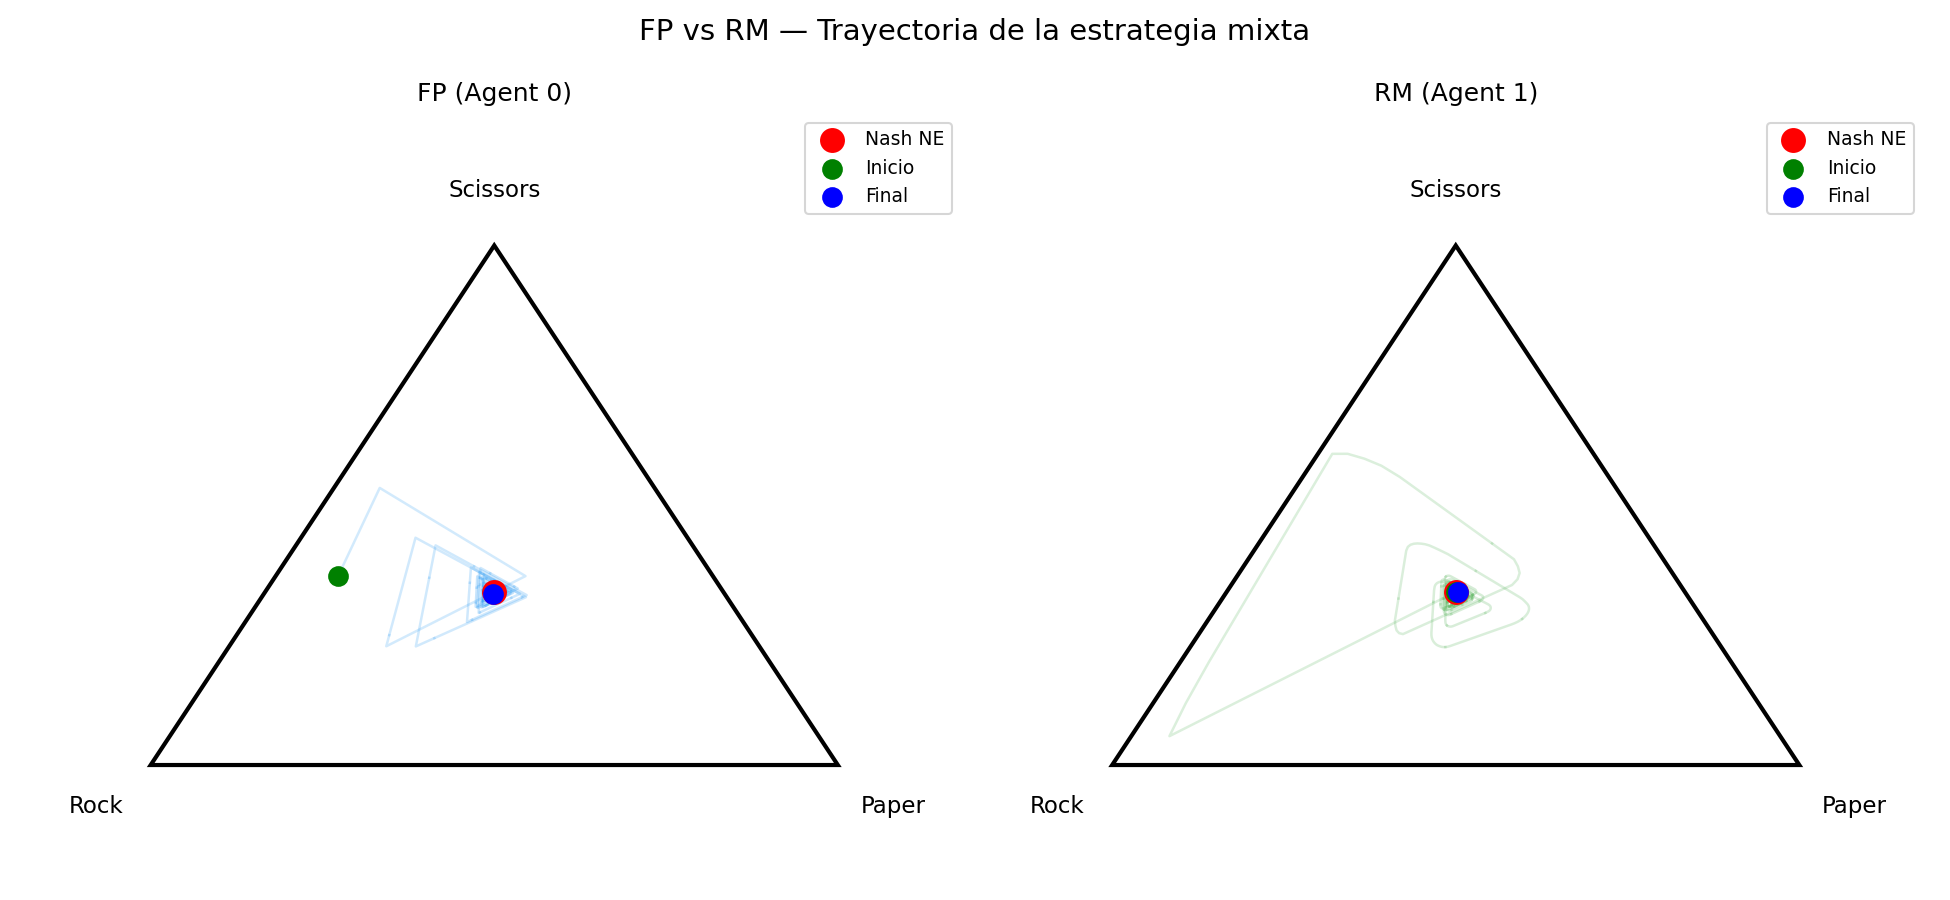
\includegraphics[width=\textwidth]{figures/RPS/simplex_fp_vs_rm.png}
    \caption{Trayectoria de políticas para FP vs RM en el simplex.}
\end{figure}

Cuando FP y RM compiten entre sí, ambos logran aproximar correctamente el equilibrio de Nash.

Las recompensas permanecen centradas alrededor de cero y las políticas promedio convergen rápidamente hacia la distribución uniforme $(1/3,1/3,1/3)$.

Puede observarse que RM parece adaptarse ligeramente más rápido durante las primeras iteraciones, mientras que FP mantiene oscilaciones más amplias. Sin embargo, en el largo plazo ambos terminan comportándose de forma muy similar.

La trayectoria de la estrategia mixta muestra además una diferencia interesante entre ambos algoritmos. FP genera movimientos más suaves y graduales alrededor del equilibrio, mientras que RM presenta curvas más pronunciadas y en algunos momentos se aleja más del centro del triángulo.

Esto ocurre porque RM ajusta directamente sus probabilidades utilizando regrets acumulados. En ciertos momentos, pequeñas diferencias en los regrets pueden provocar cambios más agresivos en la política, aumentando considerablemente la probabilidad de algunas acciones antes de volver a estabilizarse.

FP, en cambio, responde utilizando la frecuencia promedio observada del oponente, generando trayectorias más progresivas y menos abruptas.

Aun así, aunque RM a veces se aleje más instantáneamente del equilibrio, su política promedio acumulada converge más rápido que FP. Esto explica por qué RM logra mantenerse más cerca del equilibrio de Nash en promedio a pesar de presentar movimientos más curvos durante el entrenamiento.

Además, comparando este experimento con RM vs RM, puede observarse que RM parece comportarse de forma más estable cuando juega contra FP. Una posible explicación es que FP genera dinámicas más suaves y predecibles, ya que actualiza sus estrategias utilizando frecuencias promedio acumuladas. Esto produce un entorno menos agresivo para RM que cuando enfrenta otro RM, donde ambos agentes realizan ajustes rápidos basados en regrets acumulados y generan oscilaciones más fuertes simultáneamente.

Como consecuencia, al enfrentarse contra FP, RM parece estabilizarse más rápido y mantener trayectorias más concentradas alrededor del equilibrio.

\subsubsection*{Todos los algoritmos vs agente aleatorio}

\begin{figure}[H]
    \centering
    
\includegraphics[width=0.7\textwidth]{figures/RPS/vs_random_comparison.png}
    \caption{Reward promedio enfrentando a un agente aleatorio.}
\end{figure}

Todos los algoritmos logran adaptarse relativamente bien frente a un agente aleatorio.

FP obtiene los mejores resultados, lo cual tiene sentido dado que modela explícitamente la frecuencia de acciones del oponente y responde con mejores respuestas puras.

RM también logra explotar correctamente al agente aleatorio. En cambio, IQL y JAL-AM presentan resultados más variables debido a la exploración y a la naturaleza más inestable del aprendizaje por refuerzo multiagente.

\subsubsection*{Matrices de cross-play}

\begin{figure}[H]
    \centering
    \begin{minipage}{0.48\textwidth}
        \centering
        
\includegraphics[width=\textwidth]{figures/RPS/win_rate_matrix.png}
        \caption{Win rate en cross-play.}
    \end{minipage}
    \hfill
    \begin{minipage}{0.48\textwidth}
        \centering
        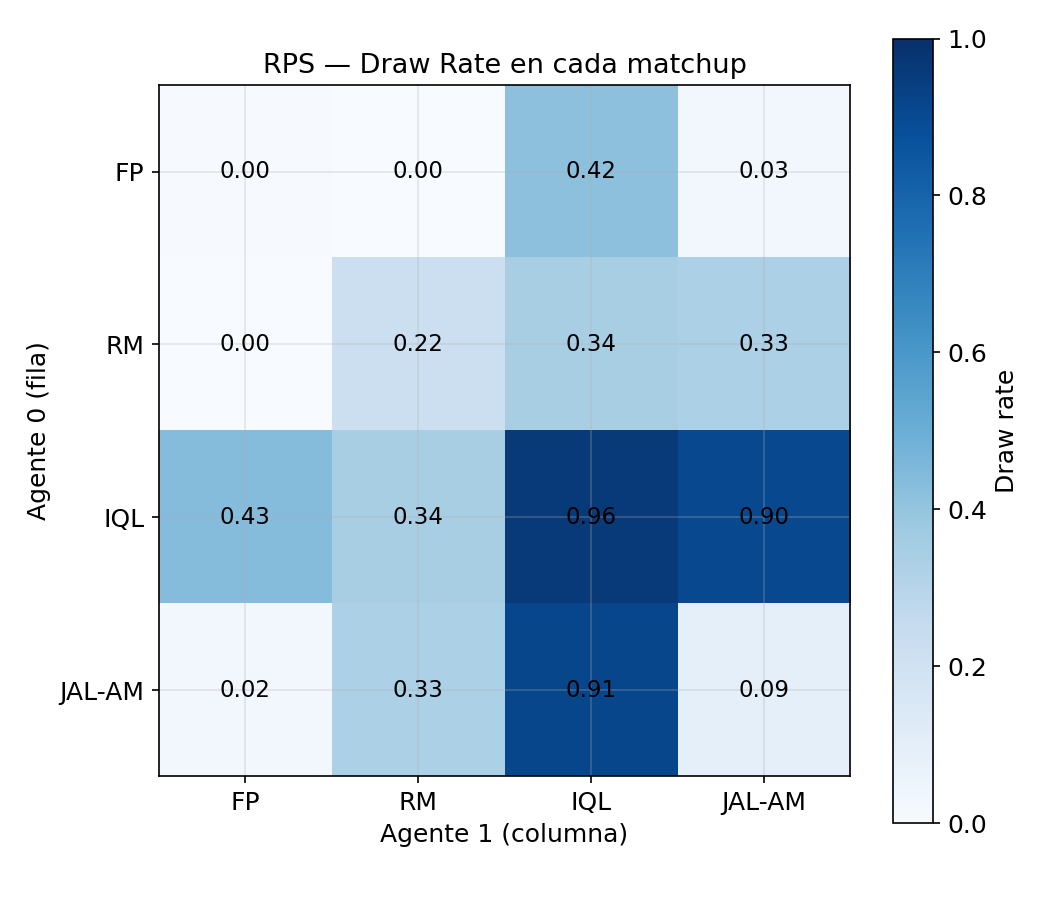
\includegraphics[width=\textwidth]{figures/RPS/draw_rate_matrix.png}
        \caption{Draw rate en cross-play.}
    \end{minipage}
\end{figure}

Las matrices de win rate y draw rate muestran resultados interesantes.

En general, FP y RM mantienen enfrentamientos relativamente balanceados entre sí, con win rates cercanas a $0.33$, consistentes con el equilibrio de Nash.

IQL presenta muchos empates cuando juega contra sí mismo, reflejando que ambos agentes terminan oscilando alrededor de políticas similares sin explotarse demasiado.

JAL-AM logra explotar bastante bien a FP, obteniendo una win rate cercana a $0.85$, probablemente porque FP mantiene patrones más predecibles de oscilación que pueden ser modelados por JAL-AM.

\subsubsection*{Distancia al equilibrio de Nash}

\begin{figure}[H]
    \centering
    
\includegraphics[width=\textwidth]{figures/RPS/all_algos_distance_ne.png}
    \caption{Distancia L1 al equilibrio de Nash.}
\end{figure}

La comparación final confirma lo observado anteriormente.

FP y RM son los algoritmos que convergen de forma más rápida y estable hacia el equilibrio de Nash. RM presenta la menor distancia sostenida al equilibrio durante gran parte del entrenamiento.

IQL es claramente el algoritmo más inestable y con mayor distancia al equilibrio. JAL-AM mejora significativamente sobre IQL gracias al modelado explícito del oponente, aunque sigue siendo más ruidoso que FP y RM.

\subsubsection*{Conclusiones}

Los experimentos realizados en Rock-Paper-Scissors muestran diferencias claras entre los algoritmos basados en teoría de juegos (FP y RM) y los algoritmos de aprendizaje por refuerzo multiagente (IQL y JAL-AM).

FP y RM fueron los algoritmos que mejor lograron aproximar el equilibrio de Nash del juego. En ambos casos, la política promedio acumulada converge claramente hacia la estrategia mixta uniforme $(1/3,1/3,1/3)$ y las recompensas permanecen centradas alrededor de cero, comportamiento esperable en un juego de suma cero.

RM fue el algoritmo más estable de todos los experimentos realizados. Las oscilaciones de sus políticas fueron menores y la convergencia hacia el equilibrio resultó más rápida que en FP. Esto también puede observarse en las trayectorias de la estrategia mixta, donde RM permanece más concentrado alrededor del centro del triangulo.

FP, por otro lado, mostró un comportamiento más gradual y suave. Sus trayectorias generan espirales más amplias alrededor del equilibrio, aunque igualmente convergen correctamente en promedio.

IQL fue claramente el algoritmo más inestable. Las políticas instantáneas continuaron fluctuando fuertemente incluso luego de miles de episodios, reflejando el problema de no estacionariedad típico del aprendizaje multiagente. Al asumir implícitamente que el entorno es estacionario, IQL tiene dificultades para adaptarse correctamente cuando el oponente también está aprendiendo y modificando continuamente su estrategia.

JAL-AM logró mejorar considerablemente respecto a IQL gracias al modelado explícito del oponente. Las políticas presentaron oscilaciones permanentes, algo esperable en un juego competitivo de suma cero como RPS, sin embargo, las trayectorias resultan más estables y cercanas al equilibrio de Nash que en IQL.

En general, los resultados muestran que:
\begin{itemize}
    \item FP y RM son especialmente adecuados para juegos simultáneos estáticos como RPS.
    \item RM fue el algoritmo más estable y con convergencia más rápida hacia el equilibrio.
    \item IQL sufre considerablemente la no estacionariedad del entorno multiagente.
    \item JAL-AM logra mitigar parcialmente este problema mediante modelado explícito del oponente.
    \item La distancia al equilibrio de Nash resulta una métrica muy útil para visualizar estabilidad y calidad de convergencia de los distintos algoritmos.
\end{itemize}

Finalmente, los experimentos muestran cómo pequeños cambios en la forma de modelar al oponente producen diferencias importantes en estabilidad y convergencia dentro de entornos multiagente competitivos.

\subsection{Foraging}

A diferencia de los juegos matriciales, el ambiente Foraging es secuencial y posee estado. Por este motivo, no se dispone de una distancia directa hacia un equilibrio de Nash conocido, sino que la evaluación combina métricas propias de aprendizaje por refuerzo con un análisis empírico de estabilidad estratégica. En particular, se consideran la recompensa promedio por episodio, la tasa de éxito, la cantidad promedio de pasos necesarios para recolectar la comida, la distribución de recompensas entre agentes y la posibilidad de que un agente mejore unilateralmente su desempeño manteniendo fijas las políticas de los demás.

En estos experimentos se evaluaron IQL y JAL-AM, ya que ambos algoritmos permiten aprender políticas dependientes del estado. Se utilizaron cuatro configuraciones con distinta complejidad:

\begin{itemize}
    \item \texttt{Foraging-5x5-2p-1f-v3}: grilla pequeña, dos agentes y un recurso.
    \item \texttt{Foraging-8x8-2p-1f-v3}: grilla más grande, dos agentes y un recurso.
    \item \texttt{Foraging-8x8-3p-1f-v3}: tres agentes, mayor complejidad de coordinación.
    \item \texttt{Foraging-8x8-3p-1f-coop-v3}: tres agentes en modo cooperativo, donde la cooperación es necesaria para recolectar el recurso.
\end{itemize}

\subsubsection*{Configuración 0: grilla 5x5 con dos agentes}

\paragraph{IQL.}\mbox{}\\

\begin{figure}[H]
    \centering
    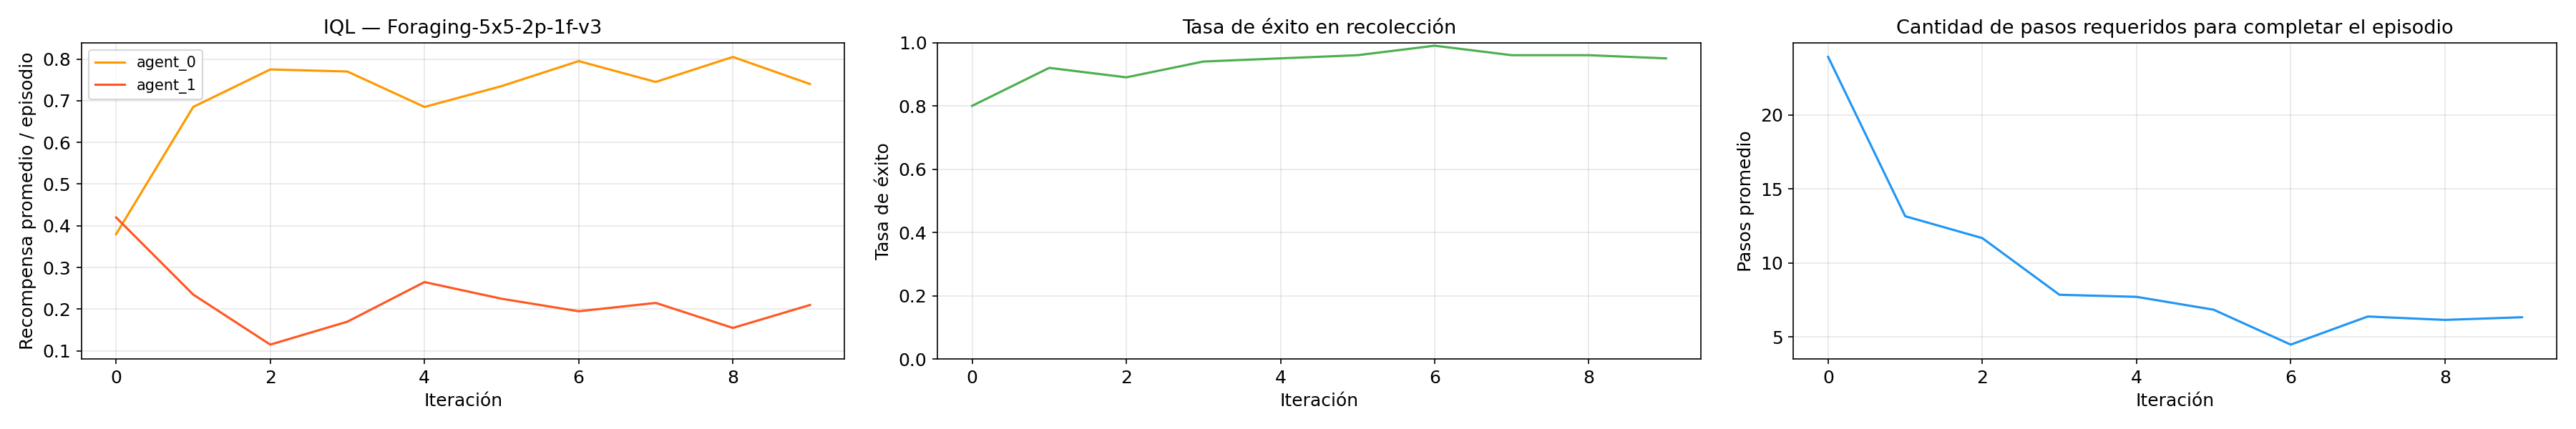
\includegraphics[width=\textwidth]{figures/Foraging/iql_config0_training.png}
    \caption{Entrenamiento de IQL en Foraging 5x5 con 2 agentes.}
\end{figure}

\begin{figure}[H]
    \centering
    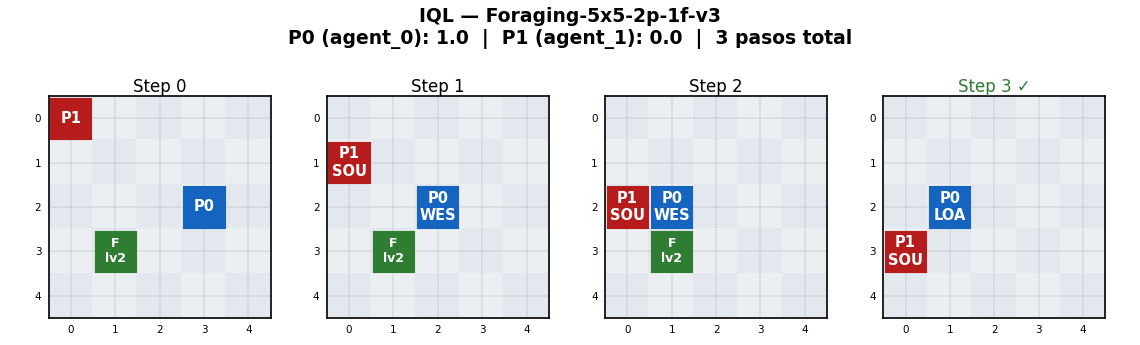
\includegraphics[width=\textwidth]{figures/Foraging/iql_config0_game.png}
    \caption{Episodio entrenado con IQL en Foraging 5x5.}
\end{figure}

En esta configuración se observa un comportamiento desbalanceado entre ambos agentes. Durante las primeras iteraciones las recompensas son relativamente similares, pero rápidamente \texttt{agent\_0} incrementa su recompensa promedio por episodio y se estabiliza en valores cercanos a $0.75 - 0.8$. En cambio, \texttt{agent\_1} reduce progresivamente su recompensa y permanece en valores considerablemente menores.

Esto sugiere que uno de los agentes aprende una política más efectiva para alcanzar o recolectar el recurso, mientras que el otro queda parcialmente desplazado durante el entrenamiento. Aun así, las recompensas se estabilizan rápido, lo cual es esperable porque la grilla es pequeña, hay un único recurso y participan solo dos agentes.

Al observar la ejecución de la política entrenada, se aprecia que ambos agentes avanzan correctamente hacia la comida y logran alcanzarla en solo 3 pasos.

\paragraph{JAL-AM.}\mbox{}\\

\begin{figure}[H]
    \centering
    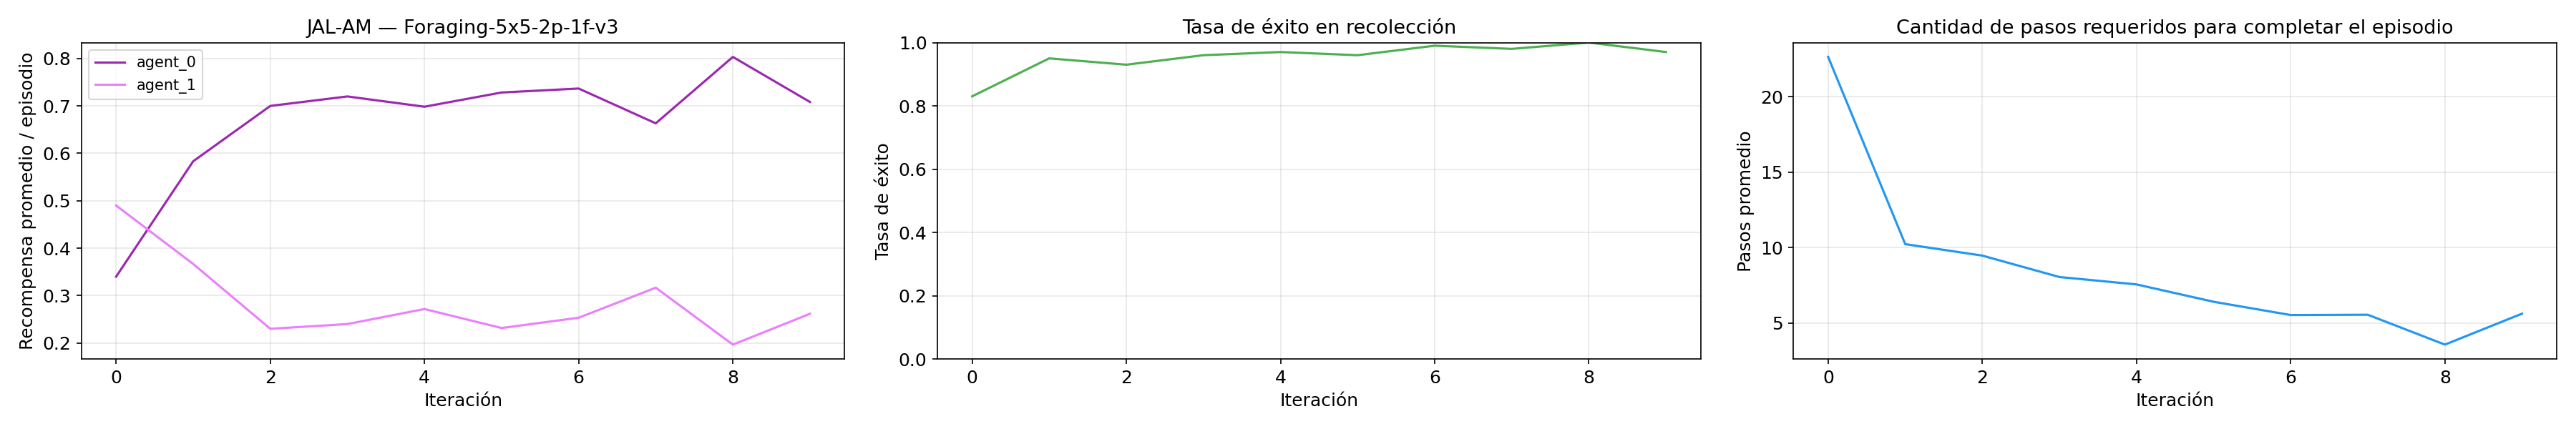
\includegraphics[width=\textwidth]{figures/Foraging/jalam_config0_training.png}
    \caption{Entrenamiento de JAL-AM en Foraging 5x5 con 2 agentes.}
\end{figure}

\begin{figure}[H]
    \centering
    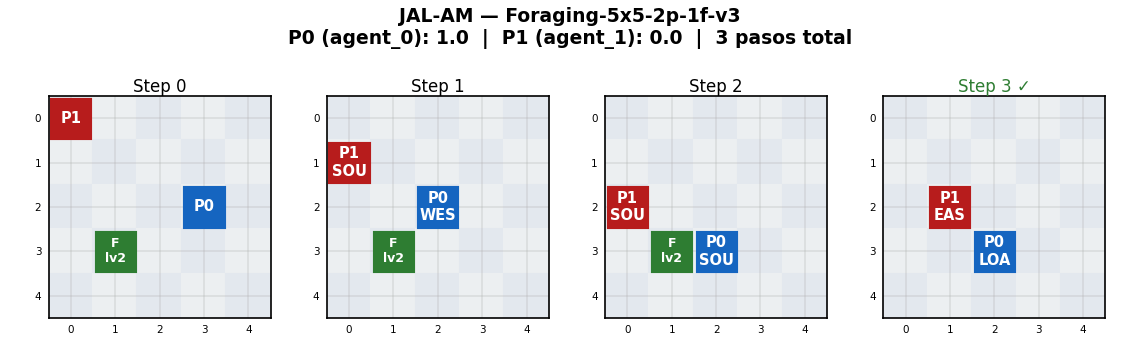
\includegraphics[width=\textwidth]{figures/Foraging/jalam_config0_game.png}
    \caption{Episodio entrenado con JAL-AM en Foraging 5x5.}
\end{figure}

En el caso de JAL-AM se observa un comportamiento similar al de IQL, pero con una evolución algo más estable durante el entrenamiento. Nuevamente, un agente incrementa rápidamente su recompensa promedio hasta valores cercanos a $0.7 - 0.8$, mientras que el otro mantiene recompensas considerablemente menores.

La principal diferencia es que las curvas presentan menos oscilaciones, lo que sugiere que el modelado explícito de las acciones de los otros agentes ayuda a estabilizar parcialmente el aprendizaje. Sin embargo, el reparto final de recompensas continúa siendo desigual, por lo que JAL-AM mejora la estabilidad pero no elimina completamente la ventaja del agente mejor posicionado.

Al observar la ejecución de la política entrenada, se aprecia que ambos agentes se desplazan de forma coordinada hacia la comida y que el recurso se recolecta exitosamente en pocos pasos.

\subsubsection*{Configuración 1: grilla 8x8 con dos agentes}

Al aumentar el tamaño de la grilla, el problema se vuelve más difícil porque los agentes necesitan explorar un espacio de estados mayor y recorrer trayectorias más largas hasta el recurso.

\paragraph{IQL.}\mbox{}\\

\begin{figure}[H]
    \centering
    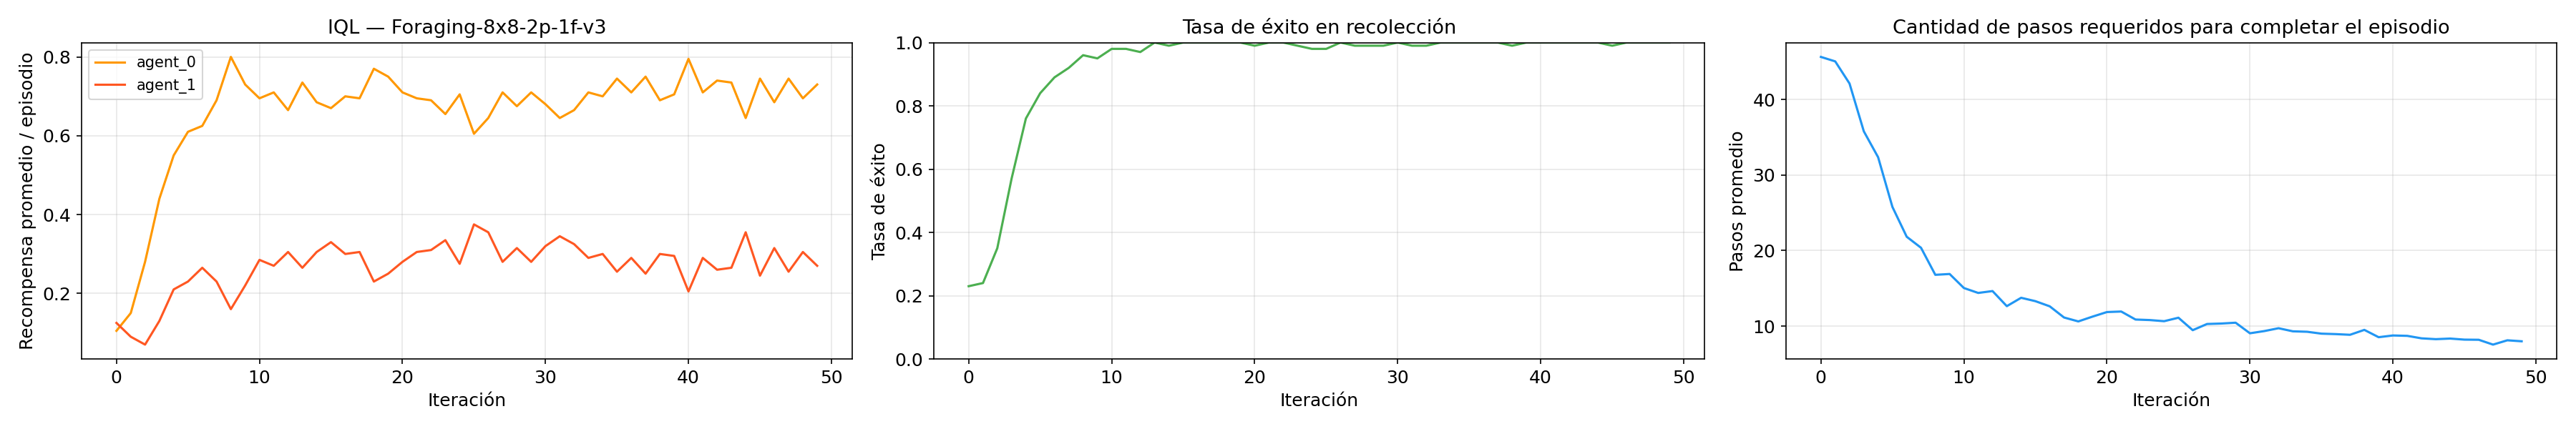
\includegraphics[width=\textwidth]{figures/Foraging/iql_config1_training.png}
    \caption{Entrenamiento de IQL en Foraging 8x8 con 2 agentes.}
\end{figure}

\begin{figure}[H]
    \centering
    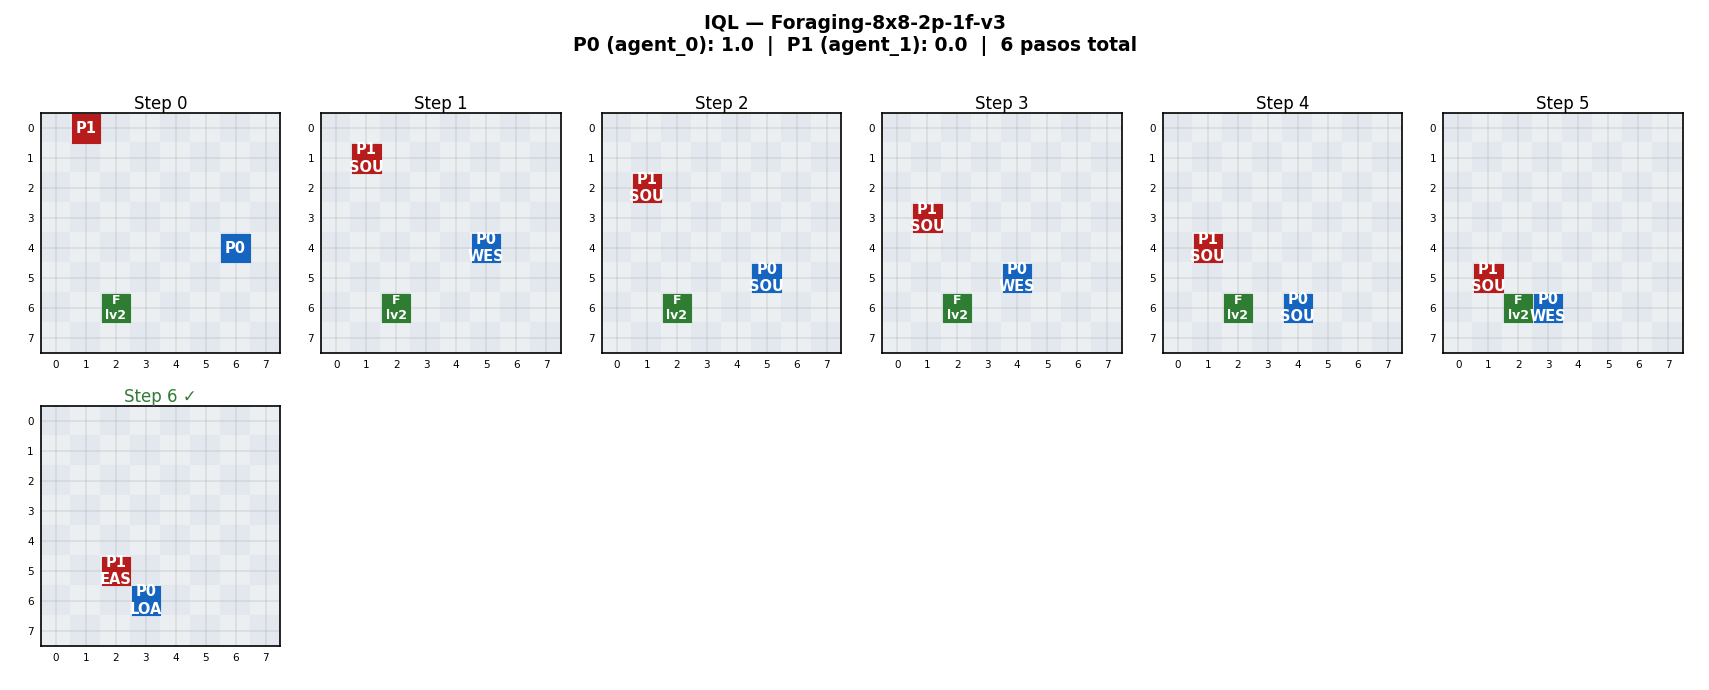
\includegraphics[width=\textwidth]{figures/Foraging/iql_config1_game.png}
    \caption{Episodio entrenado con IQL en Foraging 8x8.}
\end{figure}

IQL logra aprender una política efectiva, pero el aumento del tamaño de la grilla vuelve el aprendizaje más difícil. Las recompensas vuelven a quedar desbalanceadas: \texttt{agent\_0} alcanza valores cercanos a $0.7 - 0.8$, mientras que \texttt{agent\_1} permanece en valores menores durante gran parte del entrenamiento.

En comparación con la grilla 5x5, las curvas presentan más fluctuaciones y una convergencia más lenta al inicio. Esto es razonable, ya que el mapa 8x8 tiene un espacio de estados mayor y requiere más exploración para encontrar trayectorias efectivas hacia el recurso.

Al observar la ejecución de la política entrenada, se ve que ambos agentes se mueven hacia la comida y que \texttt{P0} logra ejecutar \texttt{LOAD} para recolectarla luego de 6 pasos.

\paragraph{JAL-AM.}\mbox{}\\

\begin{figure}[H]
    \centering
    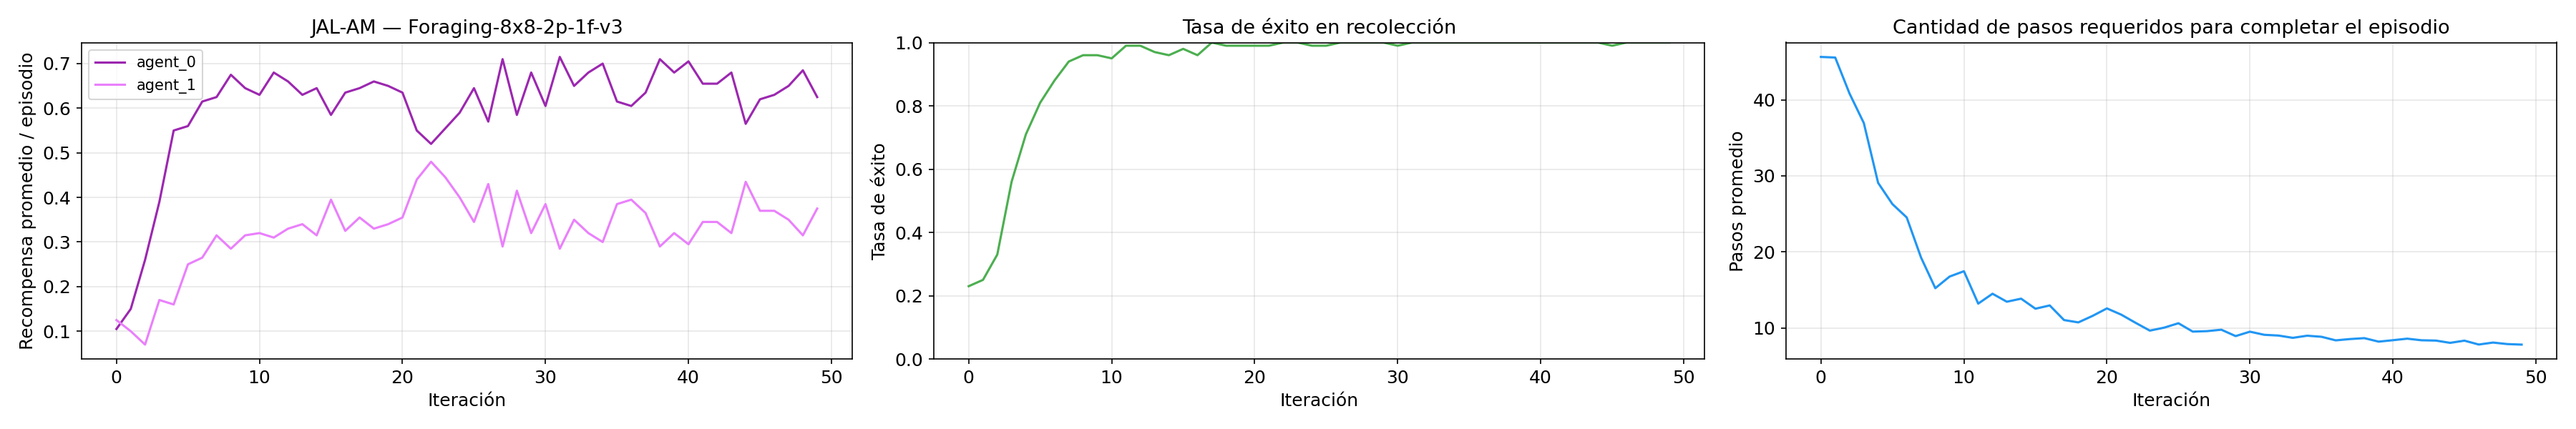
\includegraphics[width=\textwidth]{figures/Foraging/jalam_config1_training.png}
    \caption{Entrenamiento de JAL-AM en Foraging 8x8 con 2 agentes.}
\end{figure}

\begin{figure}[H]
    \centering
    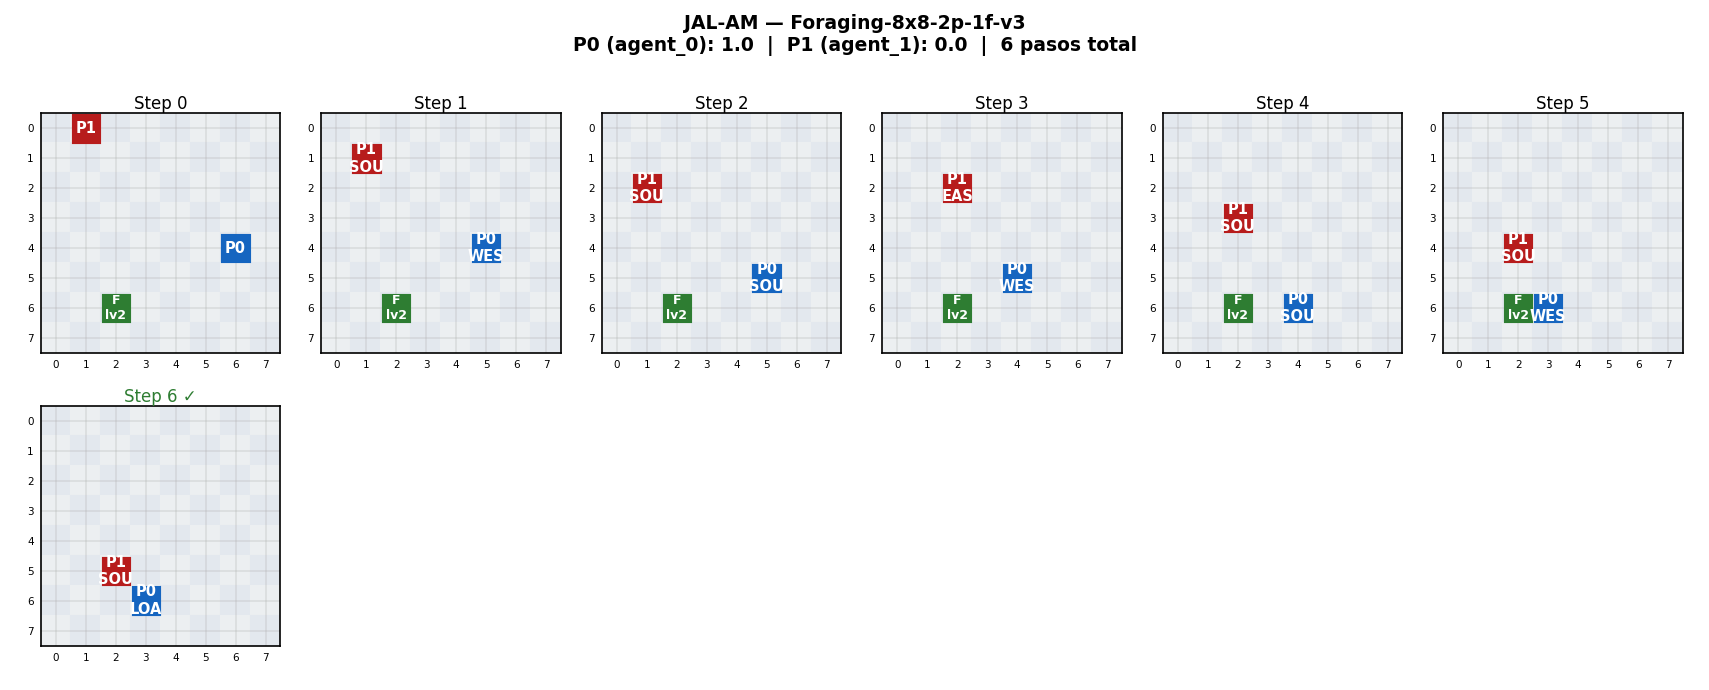
\includegraphics[width=\textwidth]{figures/Foraging/jalam_config1_game.png}
    \caption{Episodio entrenado con JAL-AM en Foraging 8x8.}
\end{figure}

JAL-AM muestra una evolución más suave que IQL en esta misma grilla. Las recompensas siguen siendo desbalanceadas, pero el segundo agente obtiene valores más altos y estables que en IQL, por lo que la diferencia entre ambos agentes es menor.

Esto sugiere que el modelado explícito del otro jugador ayuda a reducir parcialmente la no estacionariedad del entorno y permite una adaptación más estable al mapa 8x8. De todos modos, la mejora no elimina por completo las diferencias de recompensa entre agentes.

Al observar la ejecución de la política entrenada, se ve que ambos agentes se mueven correctamente hacia la comida y terminan próximos al recurso. Finalmente, \texttt{P0} ejecuta \texttt{LOAD} y recolecta la comida luego de 6 pasos. Esto indica que JAL-AM aprende una política efectiva en una grilla más grande y con trayectorias más largas.

\subsubsection*{Configuración 2: grilla 8x8 con tres agentes}

Con tres agentes aparece una dinámica de cooperación parcial. En lugar de observarse un único agente dominante, dos agentes suelen concentrar la mayor parte de la recompensa, mientras que un tercero queda relegado.

\paragraph{IQL.}\mbox{}\\

\begin{figure}[H]
    \centering
    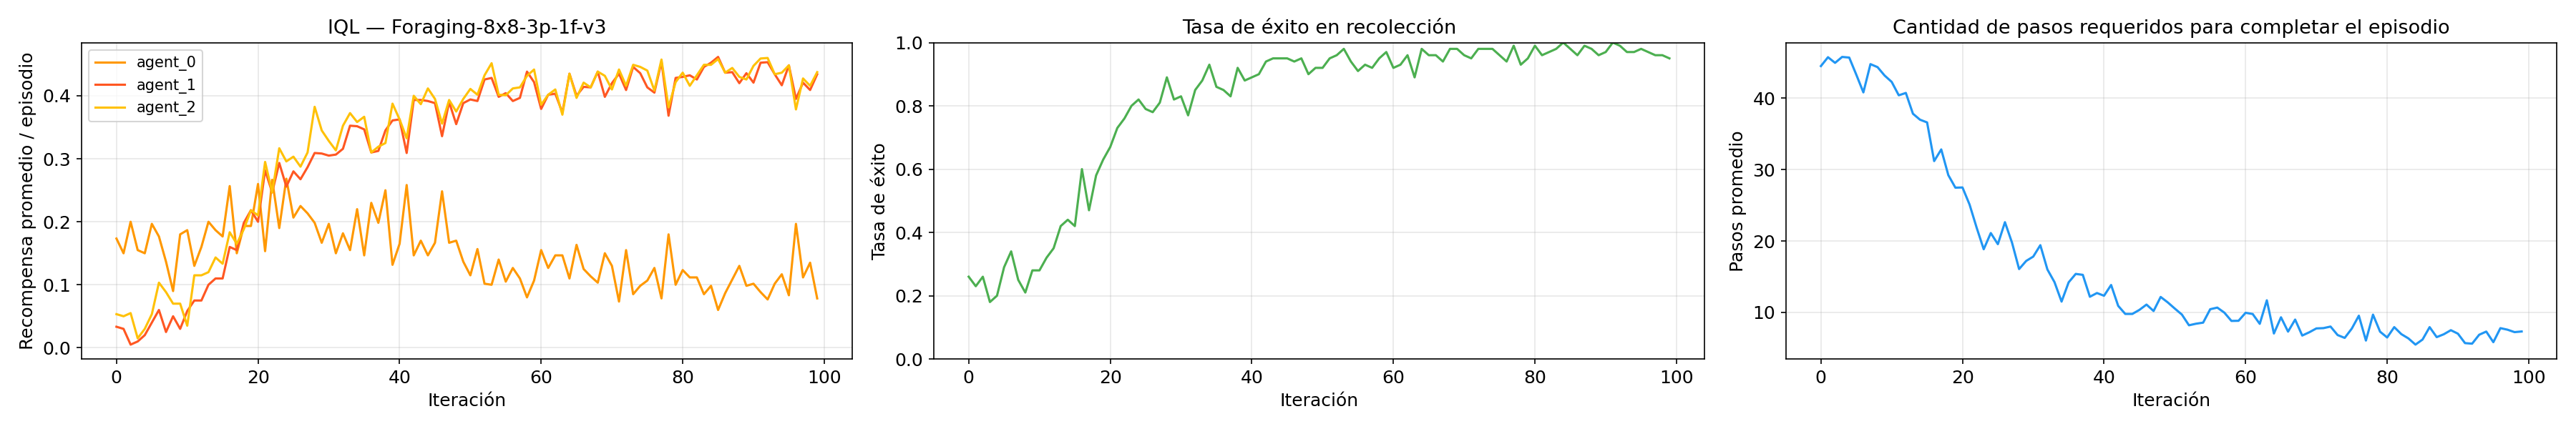
\includegraphics[width=\textwidth]{figures/Foraging/iql_config2_training.png}
    \caption{Entrenamiento de IQL en Foraging 8x8 con 3 agentes.}
\end{figure}

\begin{figure}[H]
    \centering
    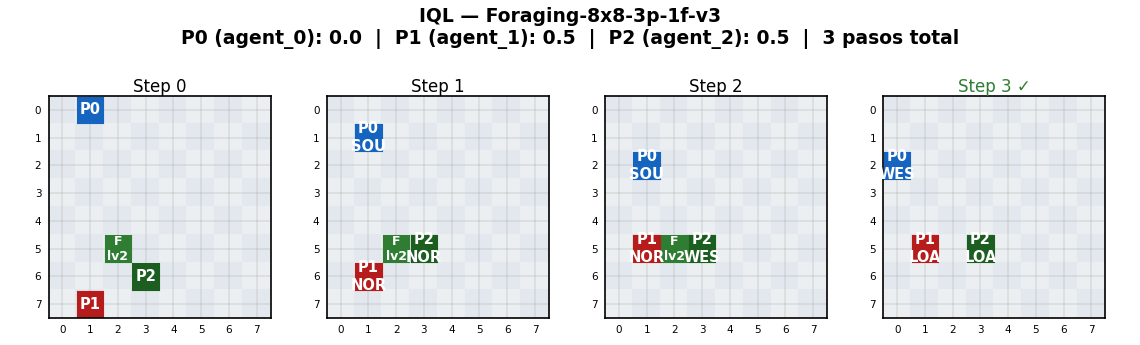
\includegraphics[width=\textwidth]{figures/Foraging/iql_config2_game.png}
    \caption{Episodio entrenado con IQL en Foraging 8x8 con 3 agentes.}
\end{figure}

Con IQL aparece una dinámica distinta a la de los escenarios con dos agentes. En lugar de concentrarse toda la recompensa en un único agente, dos agentes logran beneficiarse simultáneamente del aprendizaje, mientras que un tercero queda parcialmente desplazado. En particular, \texttt{agent\_1} y \texttt{agent\_2} alcanzan recompensas cercanas a $0.4 - 0.45$, mientras que \texttt{agent\_0} permanece en valores considerablemente menores.

Esto muestra que la presencia de un tercer agente aumenta la complejidad de coordinación. La posición inicial, la exploración temprana y la coordinación local influyen fuertemente en qué agentes terminan participando de la recolección.

Al observar la ejecución de la política entrenada, se aprecia que \texttt{P1} y \texttt{P2} se ubican cerca del recurso y ejecutan \texttt{LOAD}, mientras que \texttt{P0} queda más alejado, y el episodio se completa en solo 3 pasos.

\paragraph{JAL-AM.}\mbox{}\\

\begin{figure}[H]
    \centering
    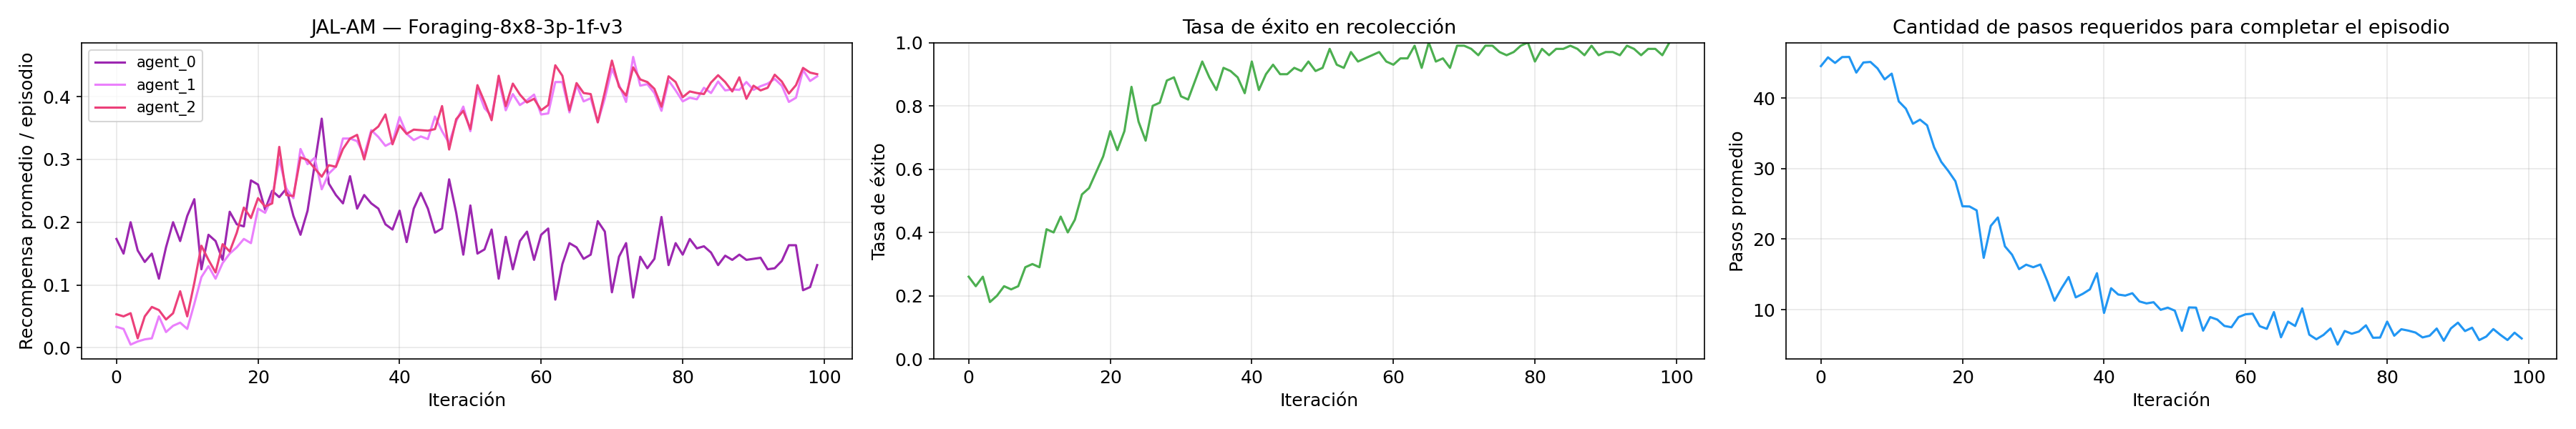
\includegraphics[width=\textwidth]{figures/Foraging/jalam_config2_training.png}
    \caption{Entrenamiento de JAL-AM en Foraging 8x8 con 3 agentes.}
\end{figure}

\begin{figure}[H]
    \centering
    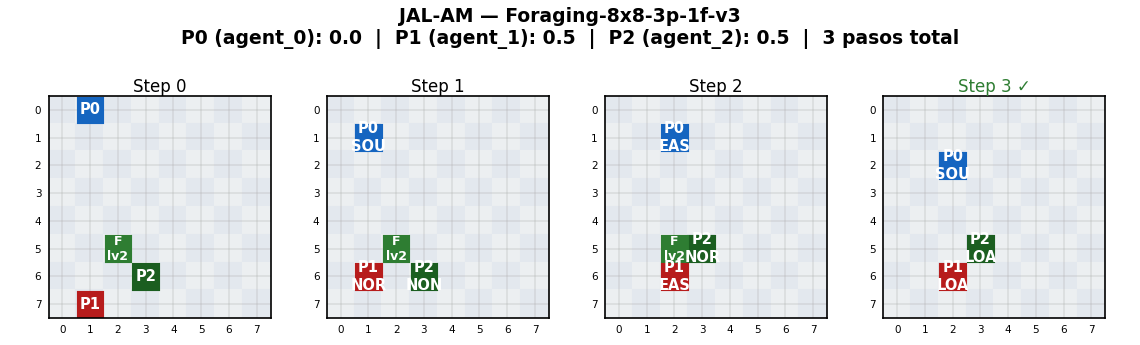
\includegraphics[width=\textwidth]{figures/Foraging/jalam_config2_game.png}
    \caption{Episodio entrenado con JAL-AM en Foraging 8x8 con 3 agentes.}
\end{figure}

Con JAL-AM aparece un patrón muy similar al observado con IQL en la misma configuración. \texttt{agent\_1} y \texttt{agent\_2} incrementan progresivamente sus recompensas hasta valores cercanos a $0.4 - 0.45$, mientras que \texttt{agent\_0} mantiene recompensas considerablemente menores durante gran parte del entrenamiento.

Las curvas son ligeramente más suaves que con IQL, pero la diferencia entre algoritmos no resulta suficientemente grande como para eliminar el desbalance. Esto sugiere que, en esta configuración, el modelado de los otros agentes mejora la estabilidad, aunque no resuelve por completo el problema de coordinación global.

Al observar la ejecución de la política entrenada, se ve que \texttt{P1} y \texttt{P2} terminan cerca del recurso y comparten la recompensa, mientras que \texttt{P0} queda más alejado. Las recompensas finales vuelven a ser aproximadamente \texttt{P0 = 0.0}, \texttt{P1 = 0.5} y \texttt{P2 = 0.5}. Esto refuerza la idea de que pequeñas diferencias de posicionamiento o exploración pueden amplificarse durante el entrenamiento y favorecer sistemáticamente a algunos agentes.

\subsubsection*{Equipos mixtos en grilla 8x8 con tres agentes}

\begin{figure}[H]
    \centering
    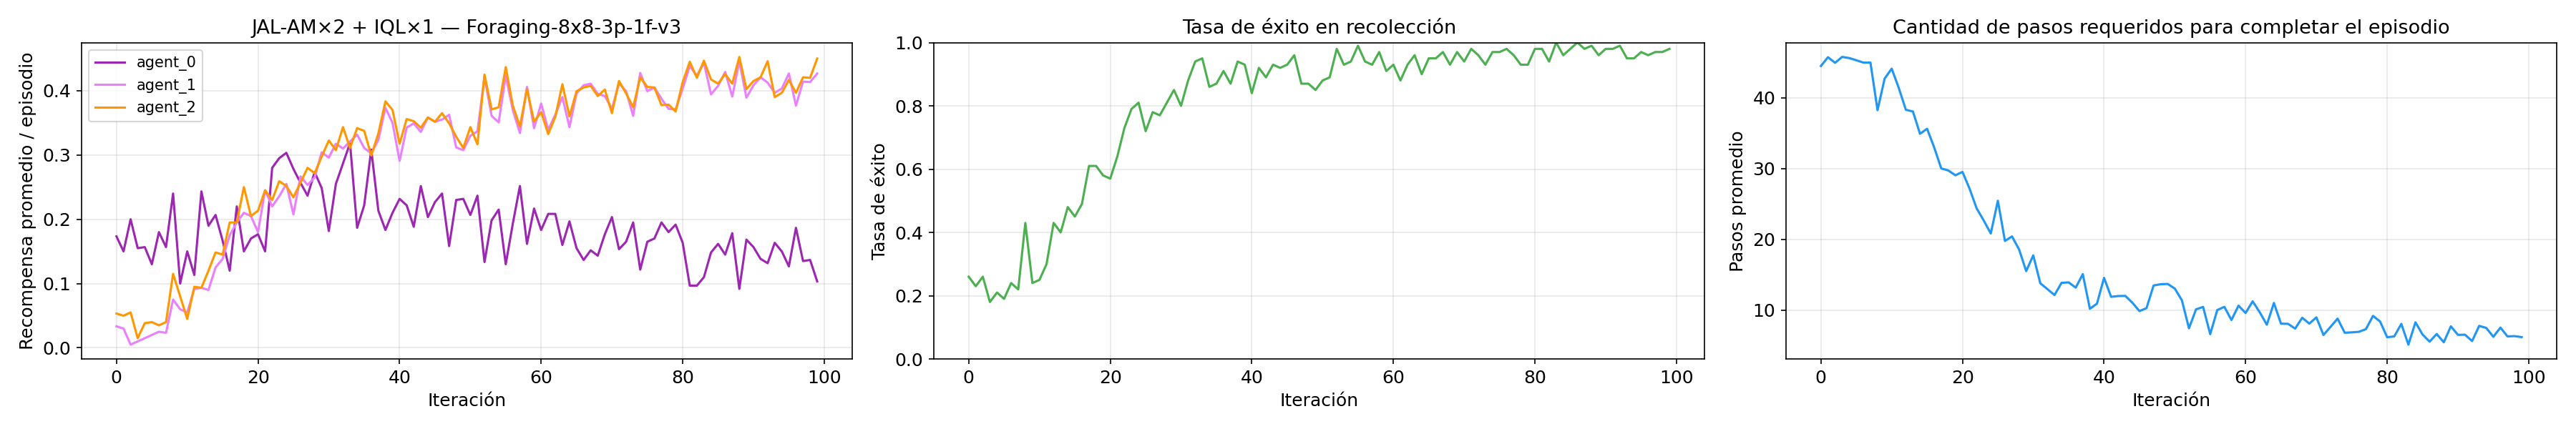
\includegraphics[width=\textwidth]{figures/Foraging/jalam2iql_config2_training.png}
    \caption{Entrenamiento de JAL-AM x2 + IQL x1 en Foraging.}
\end{figure}

\begin{figure}[H]
    \centering
    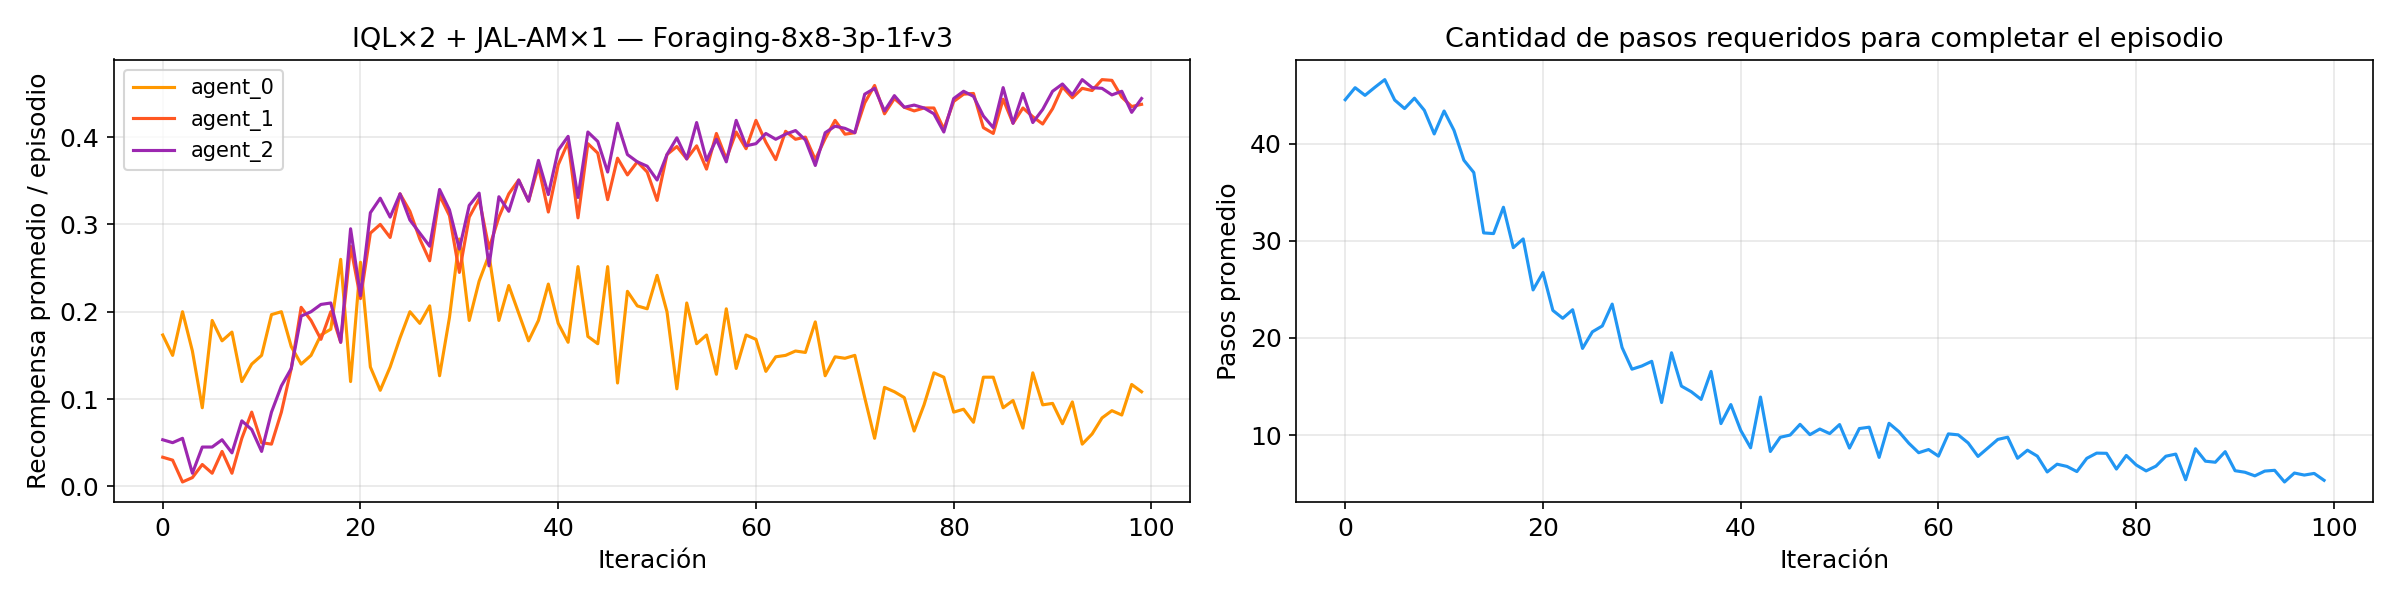
\includegraphics[width=\textwidth]{figures/Foraging/iql2jalam_config2_training.png}
    \caption{Entrenamiento de IQL x2 + JAL-AM x1 en Foraging.}
\end{figure}

\begin{figure}[H]
    \centering
    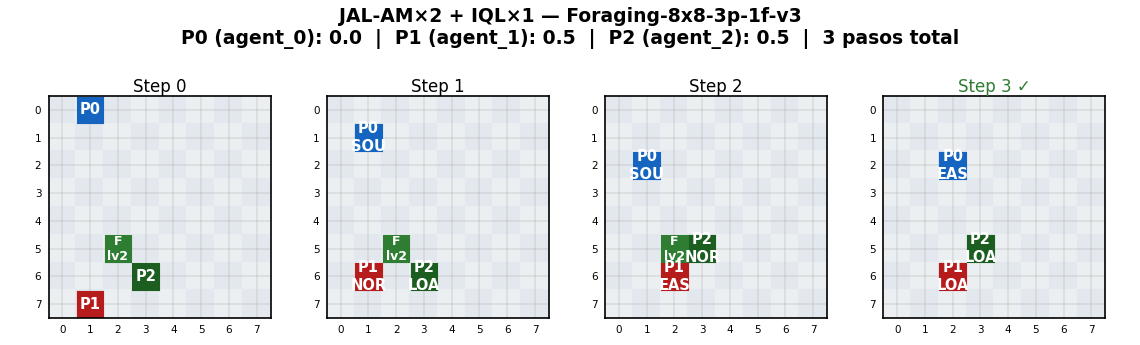
\includegraphics[width=\textwidth]{figures/Foraging/jalam2iql_config2_game.png}
    \caption{Episodio con JAL-AM x2 + IQL x1.}
\end{figure}

\begin{figure}[H]
    \centering
    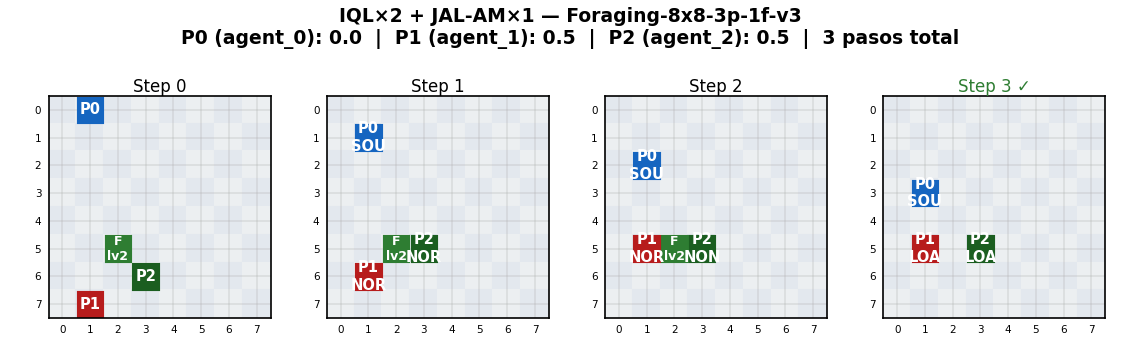
\includegraphics[width=\textwidth]{figures/Foraging/iql2jalam_config2_game.png}
    \caption{Episodio con IQL x2 + JAL-AM x1.}
\end{figure}

También se evaluaron equipos mixtos con dos agentes de un algoritmo y un agente del otro. En ambos casos se repite la estructura general observada en la configuración con tres agentes: dos agentes logran incrementar sus recompensas hasta valores cercanos a $0.4 - 0.45$, mientras que un tercero queda con recompensas muy bajas.

El agente JAL-AM no obtiene siempre una ventaja clara por el solo hecho de modelar a los demás agentes. En una de las combinaciones, el agente IQL logra recompensas similares a las de los mejores agentes del entorno; en la otra, el agente JAL-AM también queda alineado con uno de los agentes de mejor desempeño. Esto indica que el algoritmo utilizado no es el único factor determinante: la posición relativa, la exploración temprana y las trayectorias aprendidas también influyen fuertemente.

Al observar la ejecución de la política entrenada, se aprecia que los equipos mixtos también logran mover agentes hacia la comida. En particular, en el segundo step \texttt{agent\_2} ejecuta la acción \texttt{NONE}, lo que sugiere que aprendió a esperar a su compañero antes de recolectar la comida. De esta forma, ambos agentes pueden ejecutar la recolección de manera coordinada y obtener una recompensa compartida.

\subsubsection*{Configuración 3: grilla 8x8 cooperativa con tres agentes}

\paragraph{IQL.}\mbox{}\\

\begin{figure}[H]
    \centering
    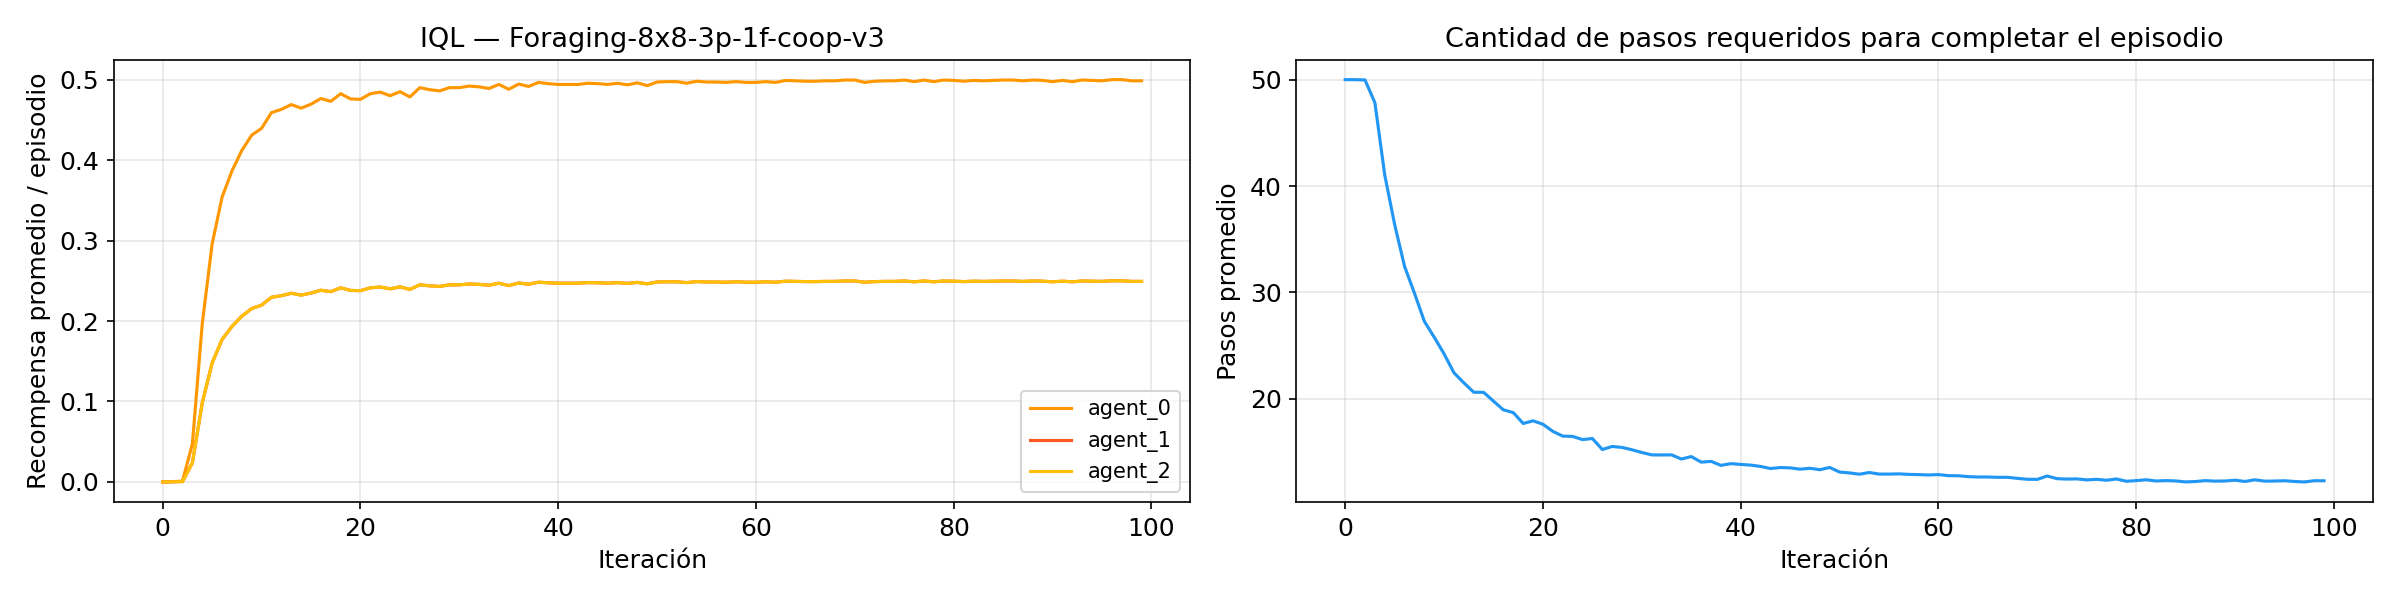
\includegraphics[width=\textwidth]{figures/Foraging/iql_config3_training.png}
    \caption{Entrenamiento de IQL en Foraging cooperativo 8x8 con 3 agentes.}
\end{figure}

\begin{figure}[H]
    \centering
    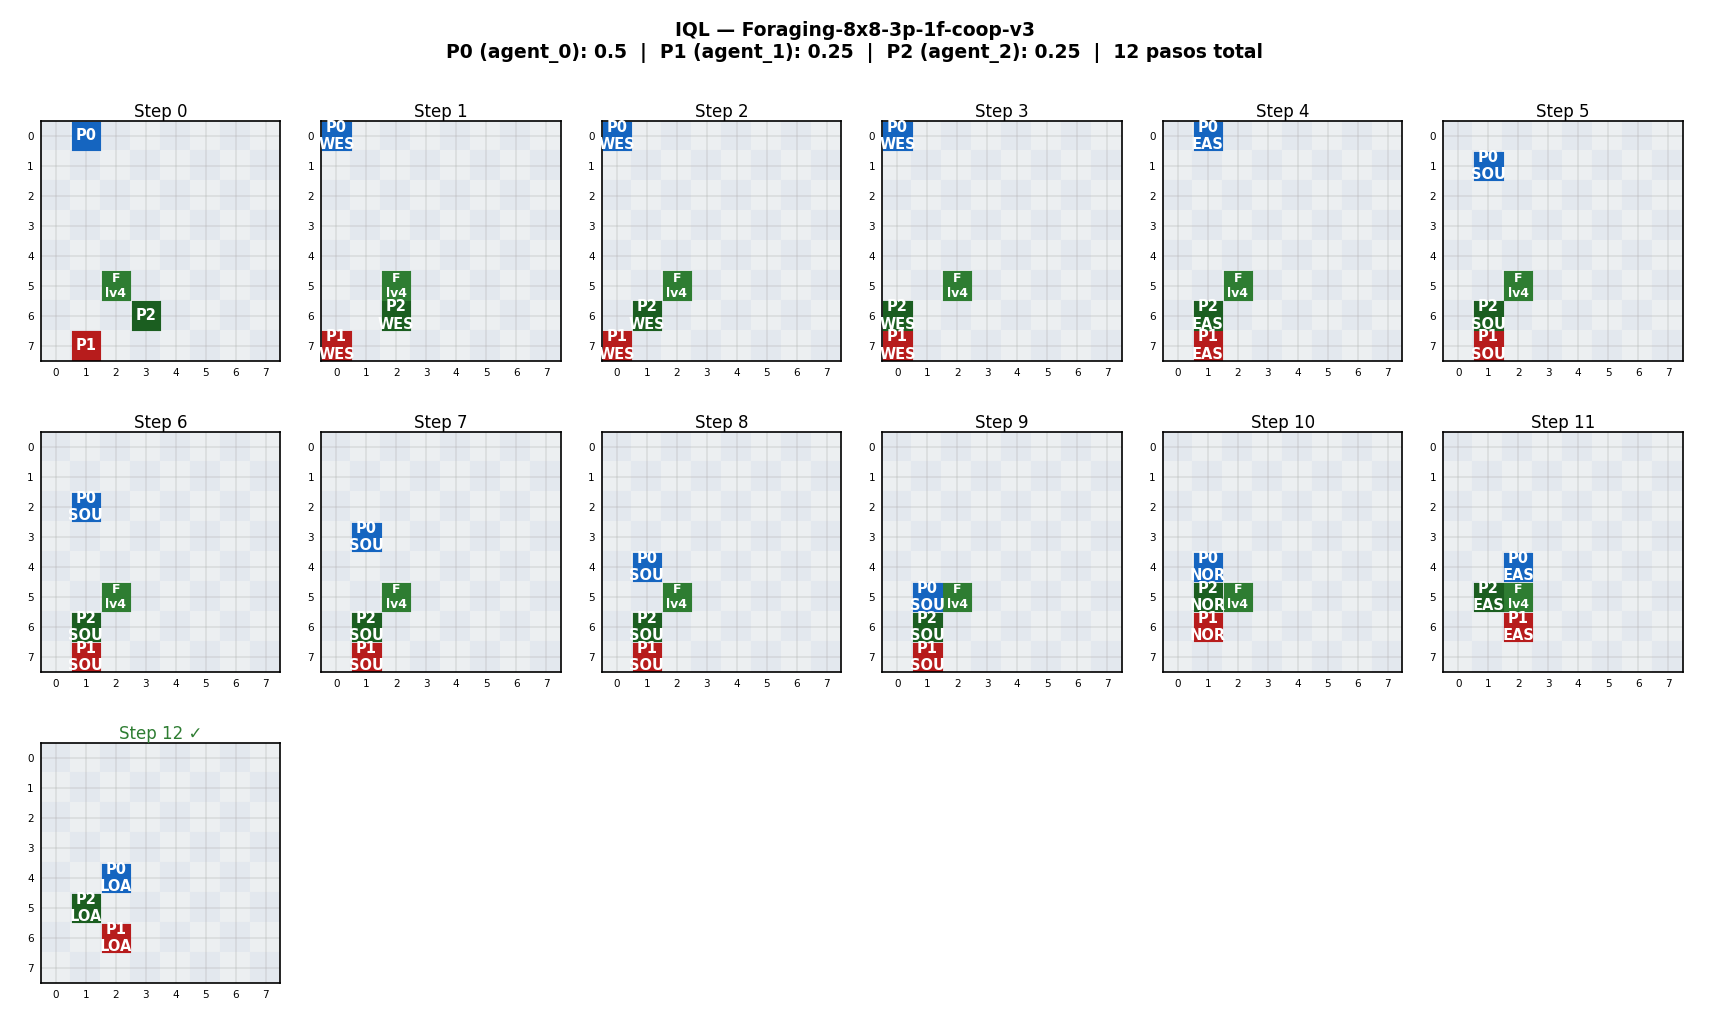
\includegraphics[width=0.75\textwidth]{figures/Foraging/iql_config3_game.png}
    \caption{Episodio entrenado con IQL en Foraging cooperativo.}
\end{figure}

En la configuración cooperativa cambia significativamente la dinámica del aprendizaje. A diferencia de los escenarios anteriores, las recompensas convergen muy rápido y luego se mantienen estables. \texttt{agent\_0} obtiene una proporción mayor, cercana a $0.5$, mientras que \texttt{agent\_1} y \texttt{agent\_2} permanecen alrededor de $0.25$.

Esta diferencia es esperada, ya que \texttt{agent\_0} tiene nivel 2, mientras que los otros dos agentes tienen nivel 1. Por lo tanto, la recompensa se distribuye de acuerdo con la contribución de cada agente: \texttt{agent\_0} recibe $0.5$ y \texttt{agent\_1} y \texttt{agent\_2} reciben $0.25$ cada uno. Es decir, todos obtienen la recompensa correspondiente a su nivel de participación.

Además, ya no aparece un agente completamente excluido. La diferencia principal es que el recurso requiere cooperación para ser recolectado, por lo que los incentivos individuales quedan más alineados con el objetivo grupal. En consecuencia, todos los agentes participan activamente del episodio y se desplazan hacia la zona del recurso.

Al observar la ejecución de la política entrenada, se ve que los agentes necesitan más pasos que en las configuraciones no cooperativas, ya que deben coordinar sus movimientos y encontrarse cerca de la comida antes de ejecutar \texttt{LOAD}. El episodio requiere alrededor de 12 pasos, lo cual es razonable porque la recolección depende de la presencia conjunta de varios agentes. Esta mayor duración refleja coordinación colectiva y no necesariamente peor desempeño.

\paragraph{JAL-AM.}\mbox{}\\

\begin{figure}[H]
    \centering
    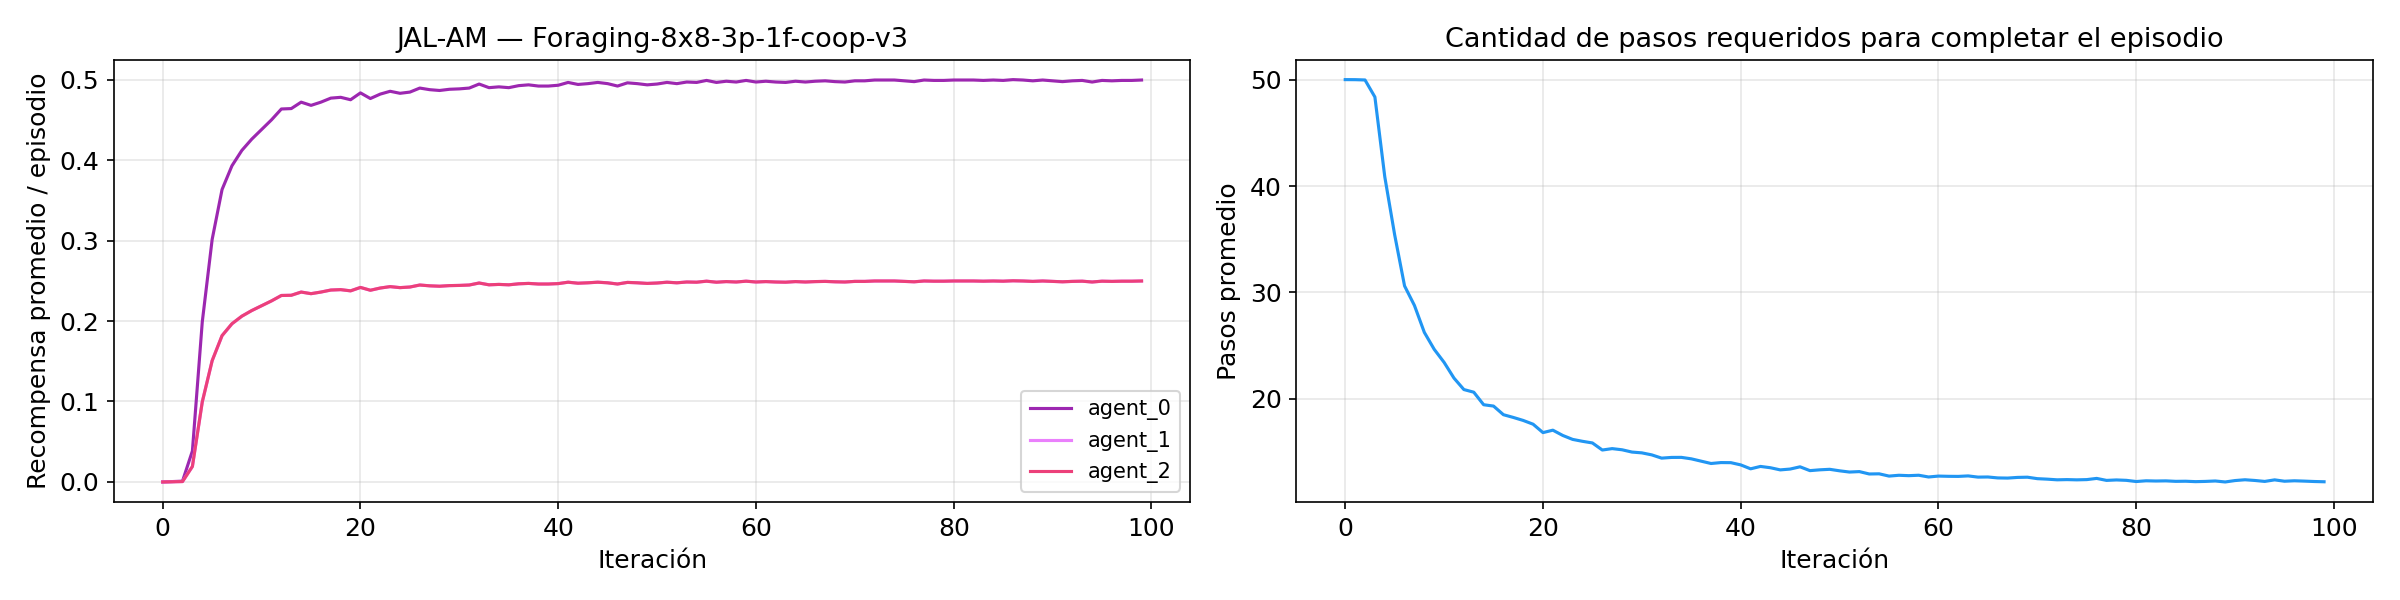
\includegraphics[width=0.75\textwidth]{figures/Foraging/jalam_config3_training.png}
    \caption{Ejecución de la política entrenada con JAL-AM en Foraging cooperativo.}
\end{figure}

\begin{figure}[H]
    \centering
    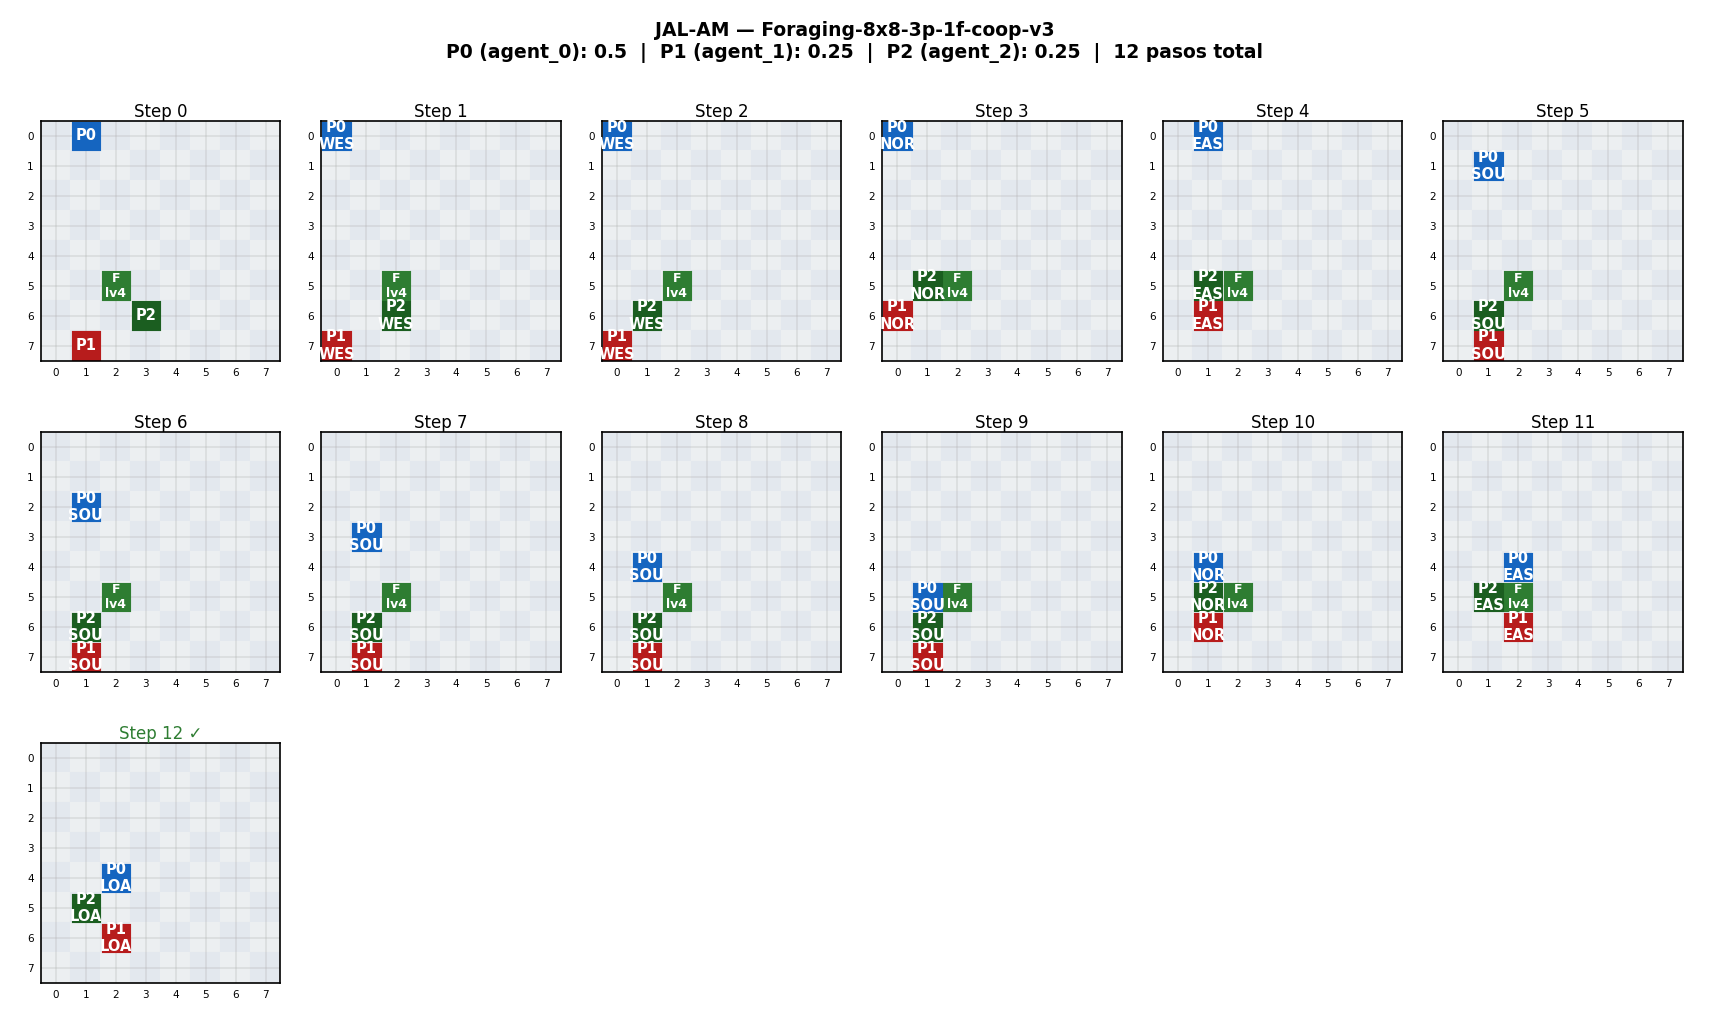
\includegraphics[width=0.75\textwidth]{figures/Foraging/jalam_config3_game.png}
    \caption{Episodio entrenado con IQL en Foraging cooperativo.}
\end{figure}

Con JAL-AM se observa un comportamiento muy similar al obtenido con IQL en la misma configuración cooperativa. Las recompensas convergen rápidamente y se mantienen estables durante el entrenamiento, con \texttt{agent\_0} cerca de $0.5$ y \texttt{agent\_1} y \texttt{agent\_2} alrededor de $0.25$.

Este patrón también es esperado por los niveles de los agentes: \texttt{agent\_0} tiene nivel 2, mientras que los otros dos agentes tienen nivel 1. Por lo tanto, la diferencia de recompensa no indica que un agente esté dominando a los demás, sino que la recompensa se reparte de acuerdo con la contribución de cada participante.

Al observar la ejecución de la política entrenada, se aprecia que los tres agentes se desplazan hacia la misma zona del mapa y permanecen relativamente agrupados cerca del recurso. Esto indica que JAL-AM también logra aprender una estrategia cooperativa efectiva, y que en este entorno el requisito de cooperación tiene un peso mayor que la diferencia entre algoritmos.

\paragraph{Entrenamientos cruzados.}\mbox{}\\

\begin{figure}[H]
    \centering
    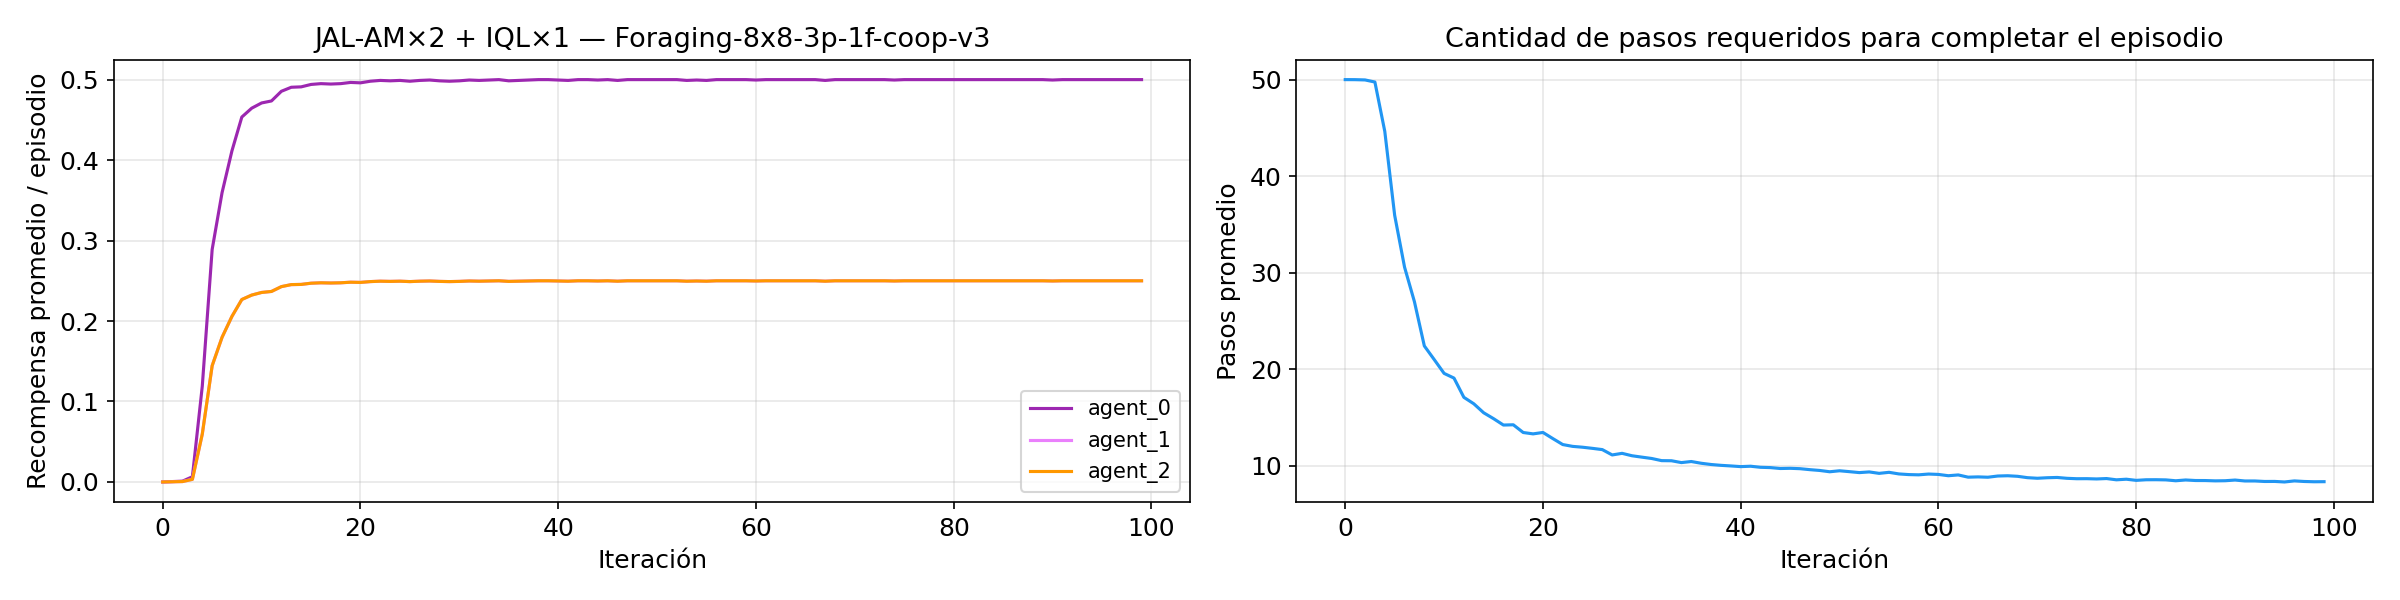
\includegraphics[width=\textwidth]{figures/Foraging/jalam2iql_config3_training.png}
    \caption{Entrenamiento de JAL-AM x2 + IQL x1 en Foraging cooperativo.}
\end{figure}

\begin{figure}[H]
    \centering
    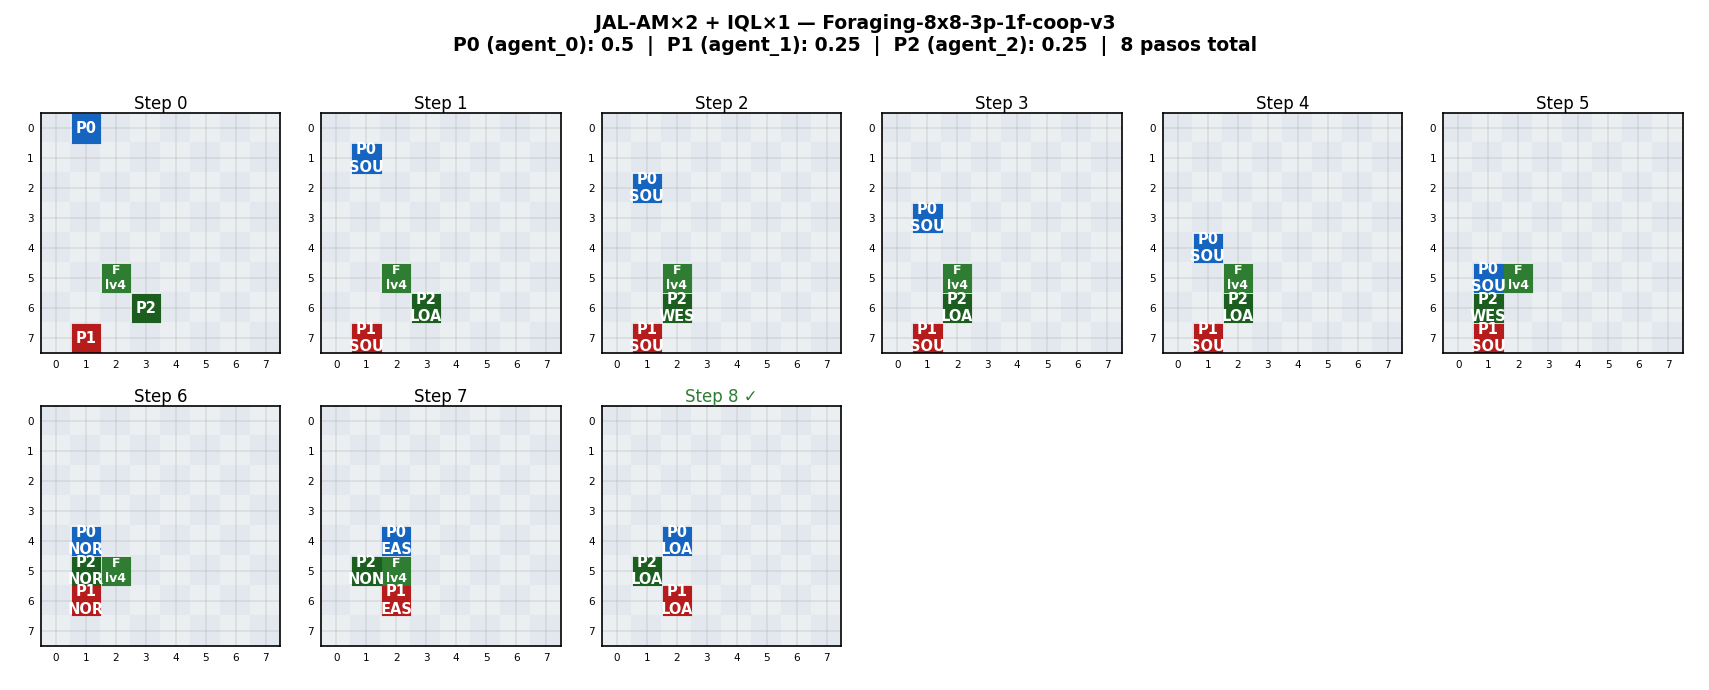
\includegraphics[width=\textwidth]{figures/Foraging/jalam2iql_config3_game.png}
    \caption{Ejecución de la política entrenada con JAL-AM x2 + IQL x1.}
\end{figure}

También se evaluaron entrenamientos cruzados, combinando agentes IQL y JAL-AM dentro del mismo equipo. Como ambos cruces presentan un comportamiento muy similar, se muestra el caso con dos agentes JAL-AM y un agente IQL como ejemplo representativo.

En este caso vuelve a aparecer una dinámica cooperativa clara: las recompensas convergen rápidamente y se distribuyen de acuerdo con los niveles de los agentes. Además, al observar la gráfica de pasos promedio, se aprecia que el equipo mixto necesita menos pasos que las configuraciones donde todos los agentes usan el mismo algoritmo. Esto sugiere que la combinación de IQL y JAL-AM puede producir trayectorias más eficientes hacia el objetivo compartido.

Al observar la ejecución de la política entrenada, se ve que los agentes convergen progresivamente hacia la comida y coordinan sus movimientos cerca del recurso. En ambos cruces, la recolección efectiva queda asociada a la cooperación entre agentes de distinto tipo, es decir, participa al menos un agente IQL y un agente JAL-AM. Por lo tanto, el resultado no parece depender únicamente de cuál algoritmo domina el equipo, sino de la coordinación que emerge entre ambos enfoques.

\subsubsection*{Conclusiones}

Los experimentos de Foraging muestran que la estructura del ambiente tiene un impacto central sobre el comportamiento emergente. En escenarios no cooperativos o mixtos, IQL y JAL-AM logran aprender trayectorias efectivas, pero las recompensas suelen distribuirse de forma desigual entre agentes. Esto ocurre especialmente cuando algunos agentes llegan antes al recurso o quedan mejor posicionados durante el entrenamiento.

Las gráficas de tasa de éxito muestran que los agentes comienzan sin poder completar el juego de forma consistente, pero luego aprenden progresivamente a recolectar la comida. Esto confirma que, aunque las recompensas no siempre se distribuyen de manera equilibrada, los algoritmos sí logran aprender políticas útiles para resolver el entorno.

Las visualizaciones de las políticas entrenadas ayudan a interpretar mejor este resultado. Por un lado, permiten comprobar que los agentes con mayor recompensa son efectivamente los que terminan ejecutando \texttt{LOAD} cerca del recurso. Por otro lado, también muestran que los agentes con menor recompensa no necesariamente aprendieron una política inútil: en varios casos se desplazan correctamente hacia la comida, pero llegan más tarde, quedan peor posicionados o no participan directamente de la acción final de recolección.

Este comportamiento es consistente con la definición teórica de los agentes. En IQL, cada agente aprende de forma independiente, por lo que una ventaja temprana de posición o exploración puede reforzarse con el tiempo. JAL-AM reduce parcialmente este problema al modelar las acciones de los demás, pero no elimina la no estacionariedad ni garantiza un reparto equilibrado.

Además, para una misma configuración los agentes comienzan siempre desde las mismas posiciones iniciales porque se utiliza el mismo \textit{seed}. Esto puede favorecer sistemáticamente a un agente si queda mejor ubicado respecto a la comida. Se realizaron pruebas adicionales rotando el \textit{seed} en cada iteración para reducir este sesgo, pero los resultados fueron peores y el desbalance se mantuvo: un agente continuó obteniendo ventaja sobre los demás. Esto sugiere que la posición inicial influye, pero no es la única causa del problema; la propia dinámica de aprendizaje multiagente también puede amplificar pequeñas diferencias tempranas.

JAL-AM tiende a producir curvas más estables que IQL, lo cual es consistente con su modelado explícito de las acciones de otros agentes. Sin embargo, esta ventaja no siempre se traduce en una distribución más equitativa de recompensas, especialmente en configuraciones con tres jugadores.

En cambio, cuando el entorno fuerza la cooperación, las diferencias entre agentes se reducen y emerge un comportamiento coordinado más claro. En este caso, la necesidad de actuar conjuntamente domina la dinámica del aprendizaje y favorece políticas donde todos los agentes participan de la recolección del recurso. Además, los experimentos cruzados en el ambiente cooperativo necesitaron menos pasos que aquellos donde todos los agentes utilizaban el mismo algoritmo, lo que sugiere que combinar IQL y JAL-AM puede favorecer trayectorias más eficientes hacia el objetivo compartido.


\section{Conclusion}

En juegos de sistemas multiagentes, el desempeño de los agentes depende fuertemente de la estructura del juego, de si es competitivo, cooperativo o mixto, y de si el entorno se mantiene estacionario mientras los agentes aprenden. Fictitious Play suele ser útil cuando el agente puede aproximar el comportamiento promedio del oponente y responder a sus frecuencias históricas, aunque puede oscilar si el rival cambia constantemente. Regret Matching tiende a ser robusto en juegos repetidos, porque ajusta su política reduciendo el arrepentimiento acumulado y puede aproximar equilibrios en términos de comportamiento promedio. IQL es simple y práctico, pero suele ser más inestable en escenarios multiagente, ya que cada agente aprende como si los demás fueran parte del entorno, ignorando que también están aprendiendo. JAL-AM, al modelar acciones conjuntas y estimar el comportamiento promedio del rival, suele capturar mejor la dependencia estratégica entre agentes que IQL, aunque también puede sufrir oscilaciones si todos los agentes adaptan sus políticas simultáneamente.

            \nocite{*}
            \bibliographystyle{apalike}
            \bibliography{Libros.bib}


%Pequeño disclaimer por si usas fotos con derechos de autor que sacaste de Internet. Nunca está de más. 
\centering \small Los créditos de las fotografías pertenecen a sus respectivos autores. ©

\centering\vspace*{\fill} 
\end{document}

 %Fin del documento.
